%! Unidad 2 — Movimiento ondulatorio (teoría, actividades resueltas y prácticas)
%! Fuente: Fuentes/Tema_2.pdf (reescrito; datos de las actividades cambiados y recalculados)

\section*{Para empezar: la ola del estadio}
\addcontentsline{toc}{section}{Para empezar: la ola del estadio}

En un estadio lleno, los espectadores de una grada se levantan y se sientan justo después de que lo hagan sus vecinos. Desde
el otro lado del campo se ve una «ola» que da la vuelta al estadio a unos \qty{12}{\m\per\second}, pero nadie se ha movido
de su asiento: cada persona solo sube y baja. Lo que viaja no son las personas, sino la \emph{perturbación}. Así funcionan
el sonido, las ondas en el agua, las cuerdas de una guitarra o la luz. En la unidad anterior estudiamos cómo vibra un punto
(el m.a.s.); en esta veremos cómo esa vibración se \textbf{propaga} de un punto a otro del espacio.

\section{¿Qué es una onda?}\label{sec:ond-concepto}

Si dejamos caer una piedra en un estanque en calma, se forman circunferencias que se alejan del punto de impacto. Las
moléculas de agua que choca la piedra empiezan a oscilar y, por las fuerzas que las unen a sus vecinas, ponen a éstas a
oscilar un poco después, y así sucesivamente. Lo mismo ocurre si agitamos el extremo de una cuerda tensa o si comprimimos
unas espiras de un muelle largo y lo soltamos.

\begin{definition}[Movimiento ondulatorio]
    Un \rojon{movimiento ondulatorio} es la propagación de una perturbación (por ejemplo, una vibración) originada en un
    punto llamado \azuln{foco}, a través de un medio o del vacío. Llamamos \rojon{onda} a la forma que adopta en cada
    instante esa perturbación.
\end{definition}

Las partículas del medio no viajan con la onda: cada una oscila alrededor de su posición de equilibrio y, cuando la
perturbación ha pasado, queda donde estaba.

\begin{remark}
    En un movimiento ondulatorio se transporta \textbf{energía} (y cantidad de movimiento), pero \textbf{no materia}. Al
    revés no es cierto: no todo transporte de energía sin materia es una onda. Al calentar un extremo de una barra metálica
    la energía llega al otro extremo por conducción, y no hay ninguna onda.
\end{remark}

\paragraph{Frentes de onda y rayos.} Para representar cómo avanza una onda se usan dos ideas geométricas
(figura~\ref{fig:ond-frentes}):
\begin{itemize}
    \item Un \azuln{frente de onda} es el conjunto de puntos del medio que, en un instante dado, tienen el mismo estado de
    vibración (la misma fase). Si el foco es puntual y el medio es igual en todas direcciones, los frentes son esferas
    (circunferencias en la superficie del agua); muy lejos del foco, un trozo pequeño de esfera es casi plano y hablamos de
    \emph{ondas planas}.
    \item Un \azuln{rayo} es una línea perpendicular a los frentes de onda que indica la dirección y el sentido de avance.
\end{itemize}

\begin{figure}[H]
    \centering
    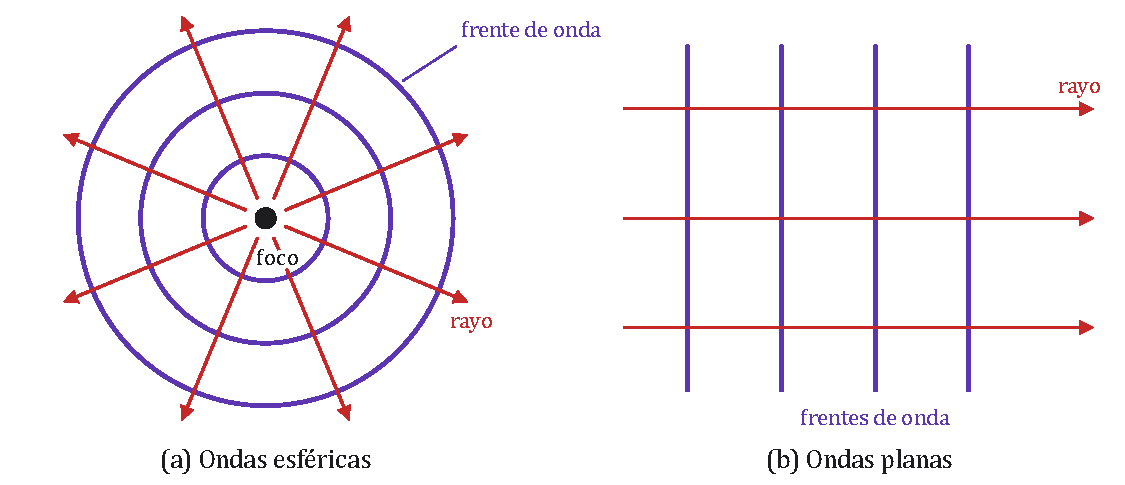
\includegraphics[width=0.85\linewidth]{images/UD2/frentes_rayos}
    \caption{Frentes de onda (en morado) y rayos (en rojo). Los rayos son siempre perpendiculares a los frentes.}
    \label{fig:ond-frentes}
\end{figure}

\section{Clasificación de las ondas}\label{sec:ond-clasificacion}

\begin{table}[H]
    \centering
    \caption{Clasificación de las ondas}
    \vspace{-5pt}
    \begin{tabular}{@{}L{3.6cm}L{3.2cm}L{6.6cm}@{}}
        \toprule
        \textbf{Criterio} & \textbf{Tipo} & \textbf{Características y ejemplos} \\
        \midrule
        \multirow{2}{3.6cm}{Duración de la perturbación} & Pulso & Perturbación breve: un golpe seco en el extremo de una cuerda. \\[3pt]
         & Tren de ondas & El foco vibra de forma continua: agitar sin parar el extremo de la cuerda. \\[3pt]
        \multirow{2}{3.6cm}{Dirección de vibración} & Longitudinales & Las partículas vibran en la dirección de propagación: muelle, sonido. \\[3pt]
         & Transversales & Vibran perpendicularmente a la propagación: cuerda, luz. \\[3pt]
        \multirow{2}{3.6cm}{Necesidad de medio} & Mecánicas & Necesitan un medio material: sonido, olas, ondas sísmicas. \\[3pt]
         & Electromagnéticas & Se propagan también en el vacío: luz, radio, rayos X. \\[3pt]
        \multirow{3}{3.6cm}{Dimensiones en que se propaga la energía} & Unidimensionales & A lo largo de una línea: cuerda, muelle. \\[3pt]
         & Bidimensionales & En una superficie: ondas en el agua. \\[3pt]
         & Tridimensionales & En todo el espacio: sonido, luz. \\
        \bottomrule
    \end{tabular}
    \label{tab:ond-clasificacion}
\end{table}

Las ondas longitudinales avanzan mediante \azuln{compresiones} (zonas donde las partículas se juntan) y
\azuln{dilataciones} (zonas donde se separan); por eso también se llaman \emph{ondas de presión}. En las transversales se
forman \azuln{crestas} y \azuln{valles} (figura~\ref{fig:ond-tipos}).

\begin{figure}[H]
    \centering
    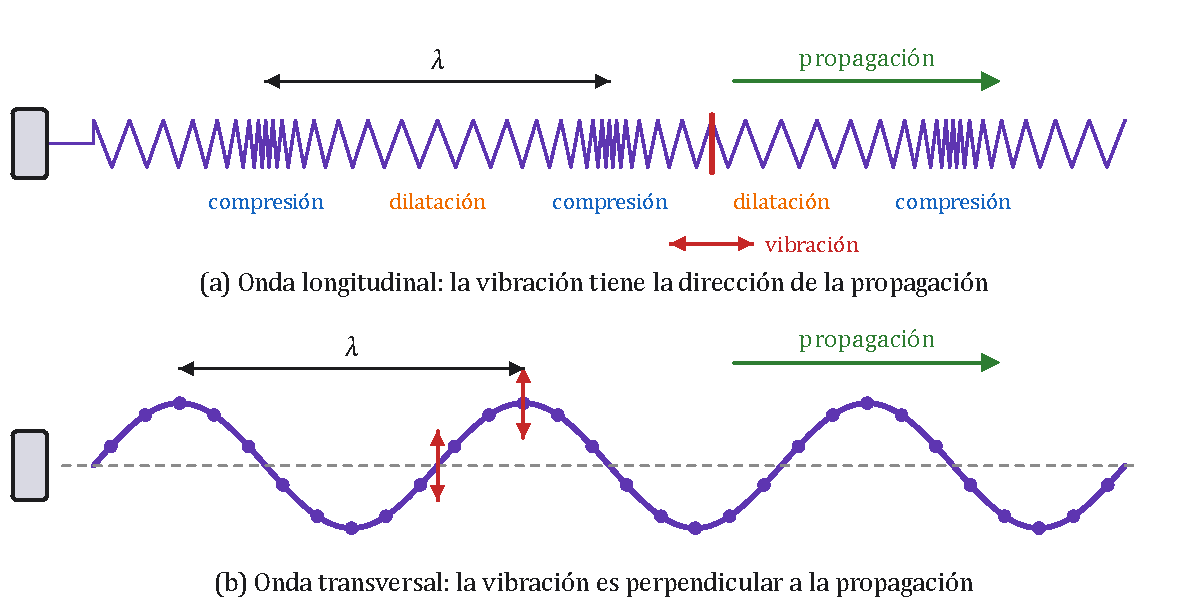
\includegraphics[width=0.95\linewidth]{images/UD2/tipos_onda}
    \caption{(a) En un muelle la vibración de cada espira tiene la misma dirección que la propagación. (b) En una cuerda cada
    punto sube y baja mientras la onda avanza en horizontal. En ambos casos \(\lambda\) es la distancia entre dos puntos que
    vibran igual.}
    \label{fig:ond-tipos}
\end{figure}

\section{Velocidad de propagación}\label{sec:ond-velocidad}

La velocidad con que avanza una onda depende \textbf{solo de las propiedades del medio} (su elasticidad y su inercia), no
de cómo vibre el foco. Si el medio es homogéneo, la velocidad es constante. Algunas expresiones (no hay que deducirlas):

\begin{table}[H]
    \centering
    \caption{Velocidad de propagación de las ondas en algunos medios}
    \vspace{-5pt}
    \begin{tabular}{@{}L{4.6cm}cL{6.4cm}@{}}
        \toprule
        \textbf{Onda} & \textbf{Velocidad} & \textbf{Magnitudes} \\
        \midrule
        Transversal en una cuerda & \(v = \sqrt{\dfrac{T}{\mu}}\) & \(T\): tensión (\unit{\newton}); \(\mu\): masa por unidad de longitud (\unit{\kg\per\m}) \\[10pt]
        Longitudinal en un muelle & \(v = l\sqrt{\dfrac{k}{m}}\) & \(k\): constante elástica; \(l\) y \(m\): longitud y masa del muelle \\[10pt]
        Longitudinal en un sólido & \(v = \sqrt{\dfrac{Y}{\rho}}\) & \(Y\): módulo de Young (\unit{\pascal}); \(\rho\): densidad \\[10pt]
        Sonido en un gas & \(v = \sqrt{\dfrac{\gamma R T}{M}}\) & \(\gamma\): coeficiente adiabático; \(T\): temperatura (\unit{\kelvin}); \(M\): masa molar (\unit{\kg\per\mol}) \\[10pt]
        Electromagnética & \(v = \dfrac{1}{\sqrt{\varepsilon\mu}}\) & \(\varepsilon\): permitividad; \(\mu\): permeabilidad magnética del medio \\
        \bottomrule
    \end{tabular}
    \label{tab:ond-velocidades}
\end{table}

Un medio en el que la onda se propagara sin perder energía sería \emph{perfectamente elástico}. Ningún medio real lo es:
el rozamiento entre partículas disipa energía y la onda se va \emph{amortiguando} (apartado~\ref{subsec:ond-amortiguacion}).

\begin{exercise}
    Una cuerda de guitarra tiene una masa de \qty{3.2}{\g} por cada metro y está tensada con una fuerza de \qty{72}{\newton}.
    Calcula la velocidad de las ondas transversales en ella. ¿Y la del sonido en el aire a \qty{20}{\celsius}?
    (\(\gamma = 1{,}4\); \(M = \qty{0.029}{\kg\per\mol}\); \(R = \qty{8.31}{\joule\per\mol\per\kelvin}\)).
    \begin{solu}
        \textcolor{blue}{Cuerda: \(\mu = \qty{3.2e-3}{\kg\per\m}\).}
        \(v = \sqrt{\dfrac{T}{\mu}} = \sqrt{\dfrac{72}{3{,}2\cdot 10^{-3}}} = \sqrt{22500} = \textcolor{red}{\qty{150}{\m\per\second}}\).

        \textcolor{blue}{Aire: \(T = \qty{293}{\kelvin}\).}
        \(v = \sqrt{\dfrac{1{,}4\cdot 8{,}31\cdot 293}{0{,}029}} = \textcolor{red}{\qty{343}{\m\per\second}}\).
    \end{solu}
\end{exercise}

\section{Magnitudes características de una onda}\label{sec:ond-magnitudes}

Pensemos en una onda armónica: el foco vibra con un m.a.s. y cada punto del medio repite ese m.a.s. con algo de retraso.

\begin{table}[H]
    \centering
    \caption{Magnitudes de una onda armónica}
    \vspace{-5pt}
    \begin{tabular}{@{}lcL{8cm}c@{}}
        \toprule
        \textbf{Magnitud} & \textbf{Símbolo} & \textbf{Significado} & \makecell{\textbf{Unidad} \\ \textbf{(SI)}} \\
        \midrule
        Elongación & \(y\) & Separación de un punto del medio respecto de su posición de equilibrio en un instante. & \unit{\m} \\[3pt]
        Amplitud & \(A\) & Elongación máxima; la misma que la del m.a.s. del foco (si no hay amortiguación). & \unit{\m} \\[3pt]
        Período & \(T\) & Tiempo que tarda cada punto en dar una vibración completa. & \unit{\second} \\[3pt]
        Frecuencia & \(\nu\) & Vibraciones por segundo de cada punto: \(\nu = 1/T\). & \unit{\hertz} \\[3pt]
        Pulsación & \(\omega\) & \(\omega = 2\pi/T = 2\pi\nu\). & \unit{\radian\per\second} \\[3pt]
        Longitud de onda & \(\lambda\) & Distancia que avanza la onda en un período. Es la distancia entre dos puntos consecutivos que vibran igual (dos crestas, dos compresiones). & \unit{\m} \\[3pt]
        Número de ondas & \(k\) & Número de longitudes de onda que caben en \(2\pi\) metros: \(k = 2\pi/\lambda\). & \unit{\per\m} \\[3pt]
        \makecell[l]{Velocidad de \\ propagación} & \(v\) & Distancia que avanza la onda por unidad de tiempo: \(v = \lambda/T = \lambda\nu\). & \unit{\m\per\second} \\
        \bottomrule
    \end{tabular}
    \label{tab:ond-magnitudes}
\end{table}

Como la onda avanza una longitud de onda en cada período:
\begin{centeredequation}
    \boxed{\lambda = v\,T = \dfrac{v}{\nu}} \qquad\qquad v = \dfrac{\omega}{k} \label{eq:ond-lambda}
\end{centeredequation}

\begin{figure}[H]
    \centering
    \begin{tikzpicture}
        \begin{axis}[fisica, width=0.8\linewidth, height=4.6cm, xmin=0, xmax=2.3, ymin=-1.5, ymax=1.6,
            xlabel={\(x\)}, ylabel={\(y\)}, xtick=\empty, ytick={-1,1}, yticklabels={\(-A\),\(A\)}]
            \addplot[domain=0:2.15, very thick, ocre] {sin(deg(2*pi*x))};
            \draw[<->, thick] (axis cs:0.25,1.3) -- node[above, font=\small]{\(\lambda\)} (axis cs:1.25,1.3);
            \draw[<->, thick] (axis cs:0.5,-1.3) -- node[below, font=\small]{\(\lambda\)} (axis cs:1.5,-1.3);
            \draw[<->, thick, blue] (axis cs:1.25,0) -- node[right, font=\small]{\(A\)} (axis cs:1.25,1);
            \draw[dashed, gray] (axis cs:0.25,1) -- (axis cs:0.25,1.3);
            \draw[dashed, gray] (axis cs:1.25,1) -- (axis cs:1.25,1.3);
            \node[font=\small, red] at (axis cs:1.75,-1.25) {valle};
            \node[font=\small, red] at (axis cs:2.05,1.25) {cresta};
        \end{axis}
    \end{tikzpicture}
    \caption{«Fotografía» de una onda transversal en un instante. La longitud de onda es la distancia entre dos crestas, dos
    valles o, en general, dos puntos consecutivos con el mismo estado de vibración.}
    \label{fig:ond-foto}
\end{figure}

\begin{remark}
    No hay que confundir dos velocidades distintas:
    \begin{itemize}
        \item la \textbf{velocidad de propagación} \(v = \lambda/T\), que es constante y depende del medio;
        \item la \textbf{velocidad de vibración} de cada partícula, \(v_y = dy/dt\), que cambia en cada instante (es la de un
        m.a.s.) y vale como máximo \(A\omega\).
    \end{itemize}
    El período, la frecuencia y la amplitud los fija el \textbf{foco}; la velocidad la fija el \textbf{medio}. La longitud
    de onda depende de los dos.
\end{remark}

\section{Ecuación de una onda armónica}\label{sec:ond-ecuacion}

La ecuación de una onda da la elongación \(y\) de cualquier punto del medio, situado a una distancia \(x\) del foco, en
cualquier instante \(t\): \(y = f(x, t)\).

Pongamos el foco en el origen, que la vibración sea en la dirección del eje \(Y\) y que la onda avance en el sentido positivo
del eje \(X\). Si el foco empieza a vibrar en su posición de equilibrio, su elongación es la de un m.a.s.:
\begin{equation*}
    y(0, t) = A\sen(\omega t)
\end{equation*}

Un punto situado a una distancia \(x\) empieza a vibrar con un retraso \(t' = x/v\), que es lo que tarda la onda en llegar
hasta él. Ese punto hace en el instante \(t\) lo mismo que hacía el foco en el instante \(t - t'\):
\begin{equation*}
    y(x, t) = y(0, t - t') = A\sen\left[\omega\left(t - \dfrac{x}{v}\right)\right]
\end{equation*}

Como \(\omega = 2\pi/T\), \(v\,T = \lambda\) y \(\omega/v = 2\pi/\lambda = k\), la misma ecuación se puede escribir de varias
formas equivalentes:
\begin{centeredequation}
    y(x,t) = A\sen\left[2\pi\left(\dfrac{t}{T} - \dfrac{x}{\lambda}\right)\right] = \boxed{A\sen(\omega t - k x)} \label{eq:ond-ecuacion}
\end{centeredequation}

\paragraph{Fase inicial.} Si en \(t = 0\) el foco no está en su posición de equilibrio, hay que añadir una fase inicial:
\begin{centeredequation}
    \boxed{y(x,t) = A\sen(\omega t - k x + \varphi_0)} \label{eq:ond-ecuacion-fase}
\end{centeredequation}
El ángulo \(\omega t - kx + \varphi_0\) es la \azuln{fase} de la onda: depende a la vez de la posición y del tiempo.

\paragraph{Sentido de propagación.} Si la onda avanza en el sentido \emph{negativo} del eje \(X\), el signo de \(kx\)
cambia:
\begin{equation*}
    y(x,t) = A\sen(\omega t + k x + \varphi_0)
\end{equation*}
Regla práctica: si \(\omega t\) y \(kx\) tienen \textbf{signos distintos}, la onda avanza hacia las \(x\) positivas; si
tienen el \textbf{mismo signo}, hacia las negativas.

\paragraph{Velocidad y aceleración de vibración.} Derivando respecto del tiempo (con \(x\) fijo):
\begin{equation*}
    v_y = \dfrac{\partial y}{\partial t} = A\omega\cos(\omega t - kx + \varphi_0) \qquad
    a_y = \dfrac{\partial v_y}{\partial t} = -A\omega^2\sen(\omega t - kx + \varphi_0) = -\omega^2 y
\end{equation*}
con valores máximos \(v_{y,\text{máx}} = A\omega\) y \(a_{y,\text{máx}} = A\omega^2\), como en un m.a.s.

\begin{exercise}
    Una onda que viaja por una cuerda tiene por ecuación, en unidades del SI, \(y = 0{,}03\sen(50t - 5x)\). Calcula la
    amplitud, la pulsación, la frecuencia, el período, la longitud de onda, la velocidad de propagación y la velocidad de
    vibración de un punto situado en \(x = \qty{20}{\cm}\) en el instante \(t = \qty{0.4}{\second}\).
    \begin{solu}
        \textcolor{blue}{Comparando con \(y = A\sen(\omega t - kx)\): \(A = \qty{0.03}{\m}\), \(\omega = \qty{50}{\radian\per\second}\), \(k = \qty{5}{\per\m}\).}

        \(\nu = \dfrac{\omega}{2\pi} = \textcolor{red}{\qty{7.96}{\hertz}}\); \(T = \dfrac{1}{\nu} = \textcolor{red}{\qty{0.126}{\second}}\);
        \(\lambda = \dfrac{2\pi}{k} = \textcolor{red}{\qty{1.26}{\m}}\); \(v = \dfrac{\omega}{k} = \textcolor{red}{\qty{10}{\m\per\second}}\).

        \textcolor{blue}{Velocidad de vibración: \(v_y = A\omega\cos(50t - 5x) = 1{,}5\cos(50t - 5x)\). En \(x = \qty{0.2}{\m}\), \(t = \qty{0.4}{\second}\) (calculadora en RAD):}
        \[ v_y = 1{,}5\cos(20 - 1) = 1{,}5\cos 19 = \textcolor{red}{\qty{1.48}{\m\per\second}} \]
    \end{solu}
\end{exercise}

\begin{exercise}
    La ecuación de una onda es \(y = 5\sen\left[10\pi\left(t - \dfrac{x}{40}\right)\right]\), con las longitudes en
    centímetros y el tiempo en segundos. Halla la amplitud, la frecuencia y la velocidad de propagación.
    \begin{solu}
        \textcolor{blue}{Comparando con \(y = A\sen\left[\omega\left(t - \dfrac{x}{v}\right)\right]\):}
        \(A = \textcolor{red}{\qty{5}{\cm}}\); \(\omega = 10\pi \Rightarrow \nu = \dfrac{10\pi}{2\pi} = \textcolor{red}{\qty{5}{\hertz}}\);
        \(v = \textcolor{red}{\qty{40}{\cm\per\second}}\).
    \end{solu}
\end{exercise}

\section{Doble periodicidad. Puntos en fase y en oposición}\label{sec:ond-periodicidad}

La ecuación de una onda es periódica respecto de dos variables:
\begin{itemize}
    \item \textbf{En el tiempo.} Si fijamos un punto (\(x\) constante) y cambiamos \(t\) por \(t + nT\), la fase aumenta en
    \(2\pi n\) y el seno no cambia: \emph{cada punto repite su estado de vibración cada período}.
    \item \textbf{En el espacio.} Si fijamos un instante (\(t\) constante) y cambiamos \(x\) por \(x + n\lambda\), la fase
    disminuye en \(2\pi n\): \emph{en cada instante, la forma de la onda se repite cada longitud de onda}.
\end{itemize}

\begin{figure}[H]
    \centering
    \begin{tikzpicture}
        \begin{axis}[fisica, width=0.47\linewidth, height=4.2cm, xmin=0, xmax=1.25, ymin=-1.35, ymax=1.5,
            xlabel={\(t\)}, ylabel={\(y\)}, xtick={0.5,1}, xticklabels={\(\frac{T}{2}\),\(T\)}, ytick={-1,1}, yticklabels={\(-A\),\(A\)},
            title={\small Un punto fijo (\(x\) constante)}]
            \addplot[domain=0:1.15, very thick, ocre] {sin(deg(2*pi*x))};
        \end{axis}
    \end{tikzpicture}\hfill
    \begin{tikzpicture}
        \begin{axis}[fisica, width=0.47\linewidth, height=4.2cm, xmin=0, xmax=1.25, ymin=-1.35, ymax=1.5,
            xlabel={\(x\)}, ylabel={\(y\)}, xtick={0.5,1}, xticklabels={\(\frac{\lambda}{2}\),\(\lambda\)}, ytick={-1,1}, yticklabels={\(-A\),\(A\)},
            title={\small Un instante fijo (\(t\) constante)}]
            \addplot[domain=0:1.15, very thick, blue] {-sin(deg(2*pi*x))};
        \end{axis}
    \end{tikzpicture}
    \caption{Doble periodicidad de una onda \(y = A\sen(\omega t - kx)\): la vibración de un punto se repite cada \(T\) y la
    forma de la onda se repite cada \(\lambda\).}
    \label{fig:ond-periodicidad}
\end{figure}

\paragraph{Concordancia y oposición de fase.} En un mismo instante, dos puntos situados en \(x_1\) y \(x_2\) tienen una
diferencia de fase:
\begin{equation*}
    \Delta\varphi = (\omega t - k x_1) - (\omega t - k x_2) = k\,(x_2 - x_1) = \dfrac{2\pi}{\lambda}\,\Delta x
\end{equation*}
\begin{itemize}
    \item Están \rojon{en fase} (misma elongación y misma velocidad) si \(\Delta\varphi = 2n\pi\), es decir, si
    \(\boxed{\Delta x = n\lambda}\): los separa un número entero de longitudes de onda.
    \item Están \rojon{en oposición de fase} (elongaciones y velocidades opuestas) si \(\Delta\varphi = (2n - 1)\pi\), es
    decir, si \(\boxed{\Delta x = (2n - 1)\,\dfrac{\lambda}{2}}\): los separa un número impar de semilongitudes de onda.
\end{itemize}
Del mismo modo, un mismo punto en dos instantes separados \(\Delta t\) tiene una diferencia de fase \(\Delta\varphi =
\omega\,\Delta t\).

\begin{exercise}
    Un foco vibra con una frecuencia de \qty{400}{\hertz} y produce ondas que se propagan a \qty{340}{\m\per\second}. Calcula:
    \begin{enumerate}[label=\letraminuscula]
        \item La distancia entre dos puntos próximos cuya diferencia de fase es \ang{60}.
        \item El tiempo que separa dos estados de vibración de un mismo punto con una diferencia de fase de \ang{180}.
        \item La diferencia de fase, en un instante dado, entre dos puntos separados \qty{2.55}{\m}.
    \end{enumerate}
    \begin{solu}
        \textcolor{blue}{\(\lambda = \dfrac{v}{\nu} = \dfrac{340}{400} = \qty{0.85}{\m}\); \(\omega = 2\pi\nu = 800\pi\ \unit{\radian\per\second}\).}
        \begin{enumerate}[label=\letraminuscula]
            \item \(\ang{60} = \dfrac{\pi}{3}\ \unit{\radian}\):
            \(\Delta x = \dfrac{\Delta\varphi}{2\pi}\,\lambda = \dfrac{\lambda}{6} = \textcolor{red}{\qty{0.142}{\m}}\).
            \item \(\Delta t = \dfrac{\Delta\varphi}{\omega} = \dfrac{\pi}{800\pi} = \textcolor{red}{\qty{1.25e-3}{\second}}\) (medio período).
            \item \(\Delta\varphi = \dfrac{2\pi}{\lambda}\,\Delta x = \dfrac{2\pi\cdot 2{,}55}{0{,}85} = \textcolor{red}{6\pi\ \unit{\radian}}\):
            \textcolor{blue}{los separan tres longitudes de onda, así que están en fase.}
        \end{enumerate}
    \end{solu}
\end{exercise}

\section{Energía e intensidad de una onda}\label{sec:ond-energia}

Cada partícula del medio vibra con un m.a.s., así que su energía es la de un oscilador
(ecuación~\eqref{eq:mas-energia}):
\begin{centeredequation}
    E = \dfrac{1}{2} k A^2 = \dfrac{1}{2} m\omega^2 A^2 = 2\pi^2 m\,\nu^2 A^2 \label{eq:ond-energia}
\end{centeredequation}
\begin{remark}
    La energía que transmite una onda es proporcional al \textbf{cuadrado de la amplitud} y al \textbf{cuadrado de la
    frecuencia}.
\end{remark}

\begin{definition}[Intensidad de una onda]
    La \rojon{intensidad} \(I\) es la energía que atraviesa, en cada unidad de tiempo, la unidad de superficie colocada
    perpendicularmente a la dirección de propagación. Es la potencia por unidad de superficie:
    \begin{centeredequation}
        \boxed{I = \dfrac{E}{S\,t} = \dfrac{P}{S}} \qquad \left[\unit{\watt\per\square\m}\right] \label{eq:ond-intensidad}
    \end{centeredequation}
\end{definition}

\paragraph{Atenuación con la distancia.} Si un foco puntual emite con potencia \(P\) en todas las direcciones y el medio no
absorbe energía, esa potencia se reparte en esferas cada vez mayores (figura~\ref{fig:ond-esferas}). A una distancia \(r\):
\begin{centeredequation}
    I = \dfrac{P}{4\pi r^2} \label{eq:ond-intensidad-r}
\end{centeredequation}

\begin{figure}[H]
    \centering
    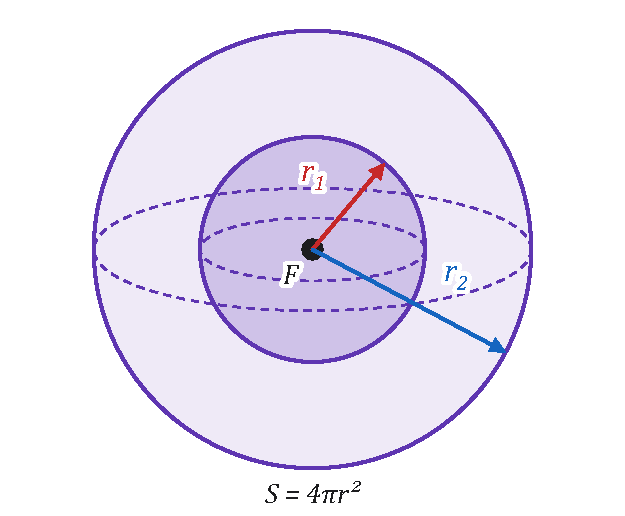
\includegraphics[width=0.38\linewidth]{images/UD2/intensidad_esferas}
    \caption{La misma potencia atraviesa las dos esferas. Como la mayor tiene más superficie, la intensidad en ella es menor.}
    \label{fig:ond-esferas}
\end{figure}

Igualando la potencia que atraviesa dos esferas de radios \(r_1\) y \(r_2\), \(I_1\,4\pi r_1^2 = I_2\,4\pi r_2^2\); y como
\(I\) es proporcional a \(A^2\):
\begin{centeredequation}
    \boxed{\dfrac{I_1}{I_2} = \dfrac{r_2^2}{r_1^2} = \dfrac{A_1^2}{A_2^2}} \qquad\Rightarrow\qquad \dfrac{A_1}{A_2} = \dfrac{r_2}{r_1} \label{eq:ond-atenuacion}
\end{centeredequation}
La intensidad disminuye con el cuadrado de la distancia y la amplitud, con la distancia.

\begin{exercise}
    Calcula la intensidad de una onda a \qty{4}{\m} de un foco puntual que emite con una potencia de \qty{60}{\watt}.
    \begin{solu}
        \(I = \dfrac{P}{4\pi r^2} = \dfrac{60}{4\pi\cdot 4^2} = \textcolor{red}{\qty{0.298}{\watt\per\square\m}}\).
    \end{solu}
\end{exercise}

\begin{exercise}
    A \qty{8}{\m} de un altavoz la intensidad del sonido es \qty{0.05}{\watt\per\square\m}. ¿Qué potencia tiene el altavoz?
    \begin{solu}
        \(P = I\cdot 4\pi r^2 = 0{,}05\cdot 4\pi\cdot 64 = \textcolor{red}{\qty{40.2}{\watt}}\).
    \end{solu}
\end{exercise}

\begin{exercise}
    Un foco emite ondas esféricas con una potencia de \qty{30}{\watt}. A \qty{3}{\m} del foco la amplitud es de \qty{2}{\cm}.
    ¿Cuánto valen la intensidad y la amplitud a \qty{6}{\m}?
    \begin{solu}
        \(I_6 = \dfrac{30}{4\pi\cdot 6^2} = \textcolor{red}{\qty{0.0663}{\watt\per\square\m}}\).
        \textcolor{blue}{Amplitud: \(\dfrac{A_6}{A_3} = \dfrac{r_3}{r_6} = \dfrac{3}{6}\)} \(\Rightarrow A_6 = \textcolor{red}{\qty{1}{\cm}}\).
        \textcolor{blue}{(Al doblar la distancia, la intensidad se divide entre 4 y la amplitud entre 2.)}
    \end{solu}
\end{exercise}

\subsection{Amortiguación}\label{subsec:ond-amortiguacion}

La amplitud de una onda disminuye al avanzar por dos causas:
\begin{itemize}
    \item \textbf{Atenuación}: en las ondas esféricas la energía se reparte entre cada vez más partículas, como acabamos de
    ver. Ocurre aunque el medio no absorba nada.
    \item \textbf{Absorción}: parte de la energía se pierde por rozamiento con las partículas del medio y se convierte en
    energía interna. La intensidad decrece exponencialmente con la distancia \(x\) recorrida en el medio:
    \begin{centeredequation}
        \boxed{I = I_0\,e^{-\beta x}} \label{eq:ond-absorcion}
    \end{centeredequation}
    donde \(I_0\) es la intensidad inicial y \(\beta\) el \azuln{coeficiente de absorción} del material (\unit{\per\m}).
\end{itemize}

\begin{exercise}
    Una onda pierde el \qty{25}{\percent} de su intensidad por absorción al atravesar \qty{8}{\cm} de un material. ¿Qué
    espesor de ese material reduce su intensidad a la mitad?
    \begin{solu}
        \textcolor{blue}{Si pierde el \qty{25}{\percent}, queda \(I = 0{,}75\,I_0\):}
        \(0{,}75 = e^{-\beta\cdot 0{,}08} \Rightarrow \beta = \dfrac{-\ln 0{,}75}{0{,}08} = \qty{3.60}{\per\m}\).

        \textcolor{blue}{Para \(I = I_0/2\):} \(x = \dfrac{\ln 2}{\beta} = \dfrac{0{,}693}{3{,}60} = \textcolor{red}{\qty{0.193}{\m} \approx \qty{19}{\cm}}\).
    \end{solu}
\end{exercise}

\section{El sonido}\label{sec:ond-sonido}

El \rojon{sonido} es una onda \textbf{mecánica}, \textbf{longitudinal} y \textbf{tridimensional}: un cuerpo vibra y produce
compresiones y dilataciones del medio que lo rodea (aire, agua, un sólido\ldots) que se propagan en todas direcciones. En el
vacío no hay sonido. Su velocidad en el aire es de unos \qty{340}{\m\per\second}; en el agua, unos \qty{1450}{\m\per\second}, y
en el acero, unos \qty{5000}{\m\per\second}.

El oído humano percibe vibraciones con frecuencias entre \qty{20}{\hertz} y \qty{20000}{\hertz}. Según la frecuencia:
\begin{itemize}
    \item \textbf{Infrasonidos}: \(\nu < \qty{20}{\hertz}\) (terremotos, algunos animales como los elefantes).
    \item \textbf{Sonidos audibles}: entre \qty{20}{\hertz} y \qty{20000}{\hertz}.
    \item \textbf{Ultrasonidos}: \(\nu > \qty{20000}{\hertz}\) (ecografías, sónar, murciélagos y delfines).
\end{itemize}

\paragraph{Eco.} El oído distingue dos sonidos como distintos si le llegan separados al menos una décima de segundo. Si un
sonido corto se refleja en un obstáculo y vuelve pasado ese tiempo, se oye repetido: es el \azuln{eco}. Con
\(v = \qty{340}{\m\per\second}\), el sonido recorre \qty{34}{\m} en \qty{0.1}{\second} (ida y vuelta), así que el obstáculo
debe estar al menos a \qty{17}{\m}. Si está más cerca, el sonido reflejado se superpone al original y lo alarga: es la
\azuln{reverberación}.

\begin{exercise}
    Al gritar frente a un acantilado oyes el eco \qty{3}{\second} después. ¿A qué distancia está? (\(v = \qty{340}{\m\per\second}\)).
    \begin{solu}
        \textcolor{blue}{El sonido va y vuelve: recorre \(2d\) en \qty{3}{\second}.}
        \(2d = 340\cdot 3 \Rightarrow d = \textcolor{red}{\qty{510}{\m}}\).
    \end{solu}
\end{exercise}

\begin{exercise}
    ¿Entre qué longitudes de onda están los sonidos que puede oír una persona? (\(v = \qty{340}{\m\per\second}\)).
    \begin{solu}
        \(\lambda = \dfrac{v}{\nu}\): \(\lambda_{\text{máx}} = \dfrac{340}{20} = \textcolor{red}{\qty{17}{\m}}\);
        \(\lambda_{\text{mín}} = \dfrac{340}{20000} = \textcolor{red}{\qty{1.7}{\cm}}\).
    \end{solu}
\end{exercise}

\begin{exercise}
    Un coche se dirige hacia una montaña a \qty{90}{\km\per\hour}, toca el claxon y recibe el eco \qty{3}{\second} después.
    ¿A qué distancia de la montaña está cuando oye el eco?
    \begin{solu}
        \textcolor{blue}{\(v_c = \qty{25}{\m\per\second}\). Sea \(d_0\) la distancia al tocar el claxon. En \qty{3}{\second} el
        sonido recorre \(340\cdot 3 = \qty{1020}{\m}\) y el coche \(25\cdot 3 = \qty{75}{\m}\). El sonido va hasta la montaña
        (\(d_0\)) y vuelve hasta el coche (\(d_0 - 75\)):}
        \[ 2d_0 - 75 = 1020 \;\Rightarrow\; d_0 = \qty{547.5}{\m} \]
        \textcolor{blue}{Al oír el eco está a} \(547{,}5 - 75 = \textcolor{red}{\qty{472.5}{\m}}\).
    \end{solu}
\end{exercise}

\begin{exercise}
    Una locomotora avanza hacia un túnel con velocidad constante. El maquinista hace sonar el silbato y oye el eco del
    túnel \qty{6}{\second} después. En ese momento vuelve a silbar y el segundo eco le llega \qty{5}{\second} más tarde.
    ¿Qué velocidad lleva? (\(v = \qty{340}{\m\per\second}\)).
    \begin{solu}
        \textcolor{blue}{Sea \(u\) la velocidad del tren y \(D\) la distancia en el primer silbido. Como en la actividad
        anterior, \(2D - 6u = 6\cdot 340\), luego \(D = 3(340 + u)\). Al segundo silbido la distancia es
        \(D' = D - 6u = 3(340 - u)\), y con el segundo eco:}
        \[ 2D' - 5u = 5\cdot 340 \;\Rightarrow\; 6\cdot 340 - 6u - 5u = 5\cdot 340 \;\Rightarrow\; 11u = 340 \]
        \(u = \textcolor{red}{\qty{30.9}{\m\per\second} \approx \qty{111}{\km\per\hour}}\).
    \end{solu}
\end{exercise}

\subsection{Cualidades del sonido}\label{subsec:ond-cualidades}

\begin{itemize}
    \item \textbf{Tono} (o altura): distingue los sonidos \emph{agudos} (frecuencia alta) de los \emph{graves} (frecuencia
    baja). Depende de la frecuencia.
    \item \textbf{Timbre}: permite distinguir la misma nota tocada por un violín y por una flauta. Un instrumento no emite
    una sola frecuencia sino la fundamental acompañada de sus armónicos (apartado~\ref{subsec:ond-armonicos}), en
    proporciones distintas; el timbre depende de la \emph{forma} de la onda.
    \item \textbf{Intensidad} (o sonoridad): distingue los sonidos fuertes de los débiles. Depende de la amplitud.
\end{itemize}

\subsection{Nivel de intensidad sonora}\label{subsec:ond-decibelios}

El oído percibe sonidos muy débiles, desde \(I_0 = \qty{e-12}{\watt\per\square\m}\) (\azuln{umbral de audición}), hasta
unos \qty{1}{\watt\per\square\m} (\azuln{umbral de dolor}): un intervalo de doce órdenes de magnitud. Además, la sensación
sonora no crece en proporción a la intensidad: un sonido de doble intensidad no se oye «el doble de fuerte». Por eso se usa
una escala logarítmica.

\begin{definition}[Nivel de intensidad sonora]
    El \rojon{nivel de intensidad sonora} (o sonoridad) \(\beta\) de un sonido de intensidad \(I\) es:
    \begin{centeredequation}
        \boxed{\beta = 10\log\dfrac{I}{I_0}} \qquad I_0 = \qty{e-12}{\watt\per\square\m} \label{eq:ond-decibelios}
    \end{centeredequation}
    Se mide en \azuln{decibelios} (\unit{\deci\bel}). El umbral de audición corresponde a \qty{0}{\deci\bel} y el de dolor a
    \qty{120}{\deci\bel}.
\end{definition}

\begin{remark}
    Cada vez que la intensidad se multiplica por 10, el nivel sube \qty{10}{\deci\bel}; si se duplica, sube \qty{3}{\deci\bel}.
    Para despejar la intensidad: \(I = I_0\cdot 10^{\beta/10}\).
\end{remark}

\begin{exercise}
    ¿Qué nivel de intensidad sonora tiene un sonido de \qty{0.5}{\watt\per\square\m}?
    \begin{solu}
        \(\beta = 10\log\dfrac{0{,}5}{10^{-12}} = 10\log(5\cdot 10^{11}) = \textcolor{red}{\qty{117}{\deci\bel}}\),
        \textcolor{blue}{muy cerca del umbral de dolor.}
    \end{solu}
\end{exercise}

\begin{exercise}
    En una discoteca se miden \qty{105}{\deci\bel}. ¿Cuál es la intensidad sonora media?
    \begin{solu}
        \(I = I_0\cdot 10^{\beta/10} = 10^{-12}\cdot 10^{10{,}5} = \textcolor{red}{\qty{0.0316}{\watt\per\square\m}}\).
    \end{solu}
\end{exercise}

\begin{exercise}
    Demuestra que un sonido de \qty{80}{\deci\bel} es mil veces más intenso que uno de \qty{50}{\deci\bel}.
    \begin{solu}
        \textcolor{blue}{Restando los niveles:}
        \[ \beta_1 - \beta_2 = 10\log\dfrac{I_1}{I_0} - 10\log\dfrac{I_2}{I_0} = 10\log\dfrac{I_1}{I_2} = 80 - 50 = 30 \]
        \(\log\dfrac{I_1}{I_2} = 3 \Rightarrow \textcolor{red}{I_1 = 1000\,I_2}\).
    \end{solu}
\end{exercise}

\paragraph{Contaminación acústica.} Llamamos \emph{ruido} a los sonidos desagradables, formados por frecuencias sin relación
entre sí. Se mide con un \emph{sonómetro}, que da el nivel en decibelios. Estar mucho tiempo expuesto a niveles altos,
aunque no lleguen al umbral de dolor, produce pérdida progresiva de audición, estrés, falta de concentración, irritabilidad o
insomnio. La Organización Mundial de la Salud recomienda no superar unos \qty{55}{\deci\bel} de día y \qty{35}{\deci\bel} de
noche en las viviendas, y se habla de contaminación acústica cuando el nivel ambiental supera los \qty{70}{\deci\bel} durante
mucho tiempo.

\begin{table}[H]
    \centering
    \caption{Niveles de intensidad sonora aproximados}
    \vspace{-5pt}
    \begin{tabular}{@{}lcc@{}}
        \toprule
        \textbf{Fuente sonora} & \textbf{Nivel (\unit{\deci\bel})} & \textbf{Intensidad (\unit{\watt\per\square\m})} \\
        \midrule
        Umbral de audición & 0 & \num{e-12} \\[3pt]
        Biblioteca, casa tranquila & 40 & \num{e-8} \\[3pt]
        Conversación normal & 60 & \num{e-6} \\[3pt]
        Calle con mucho tráfico & 80 & \num{e-4} \\[3pt]
        Concierto, discoteca & 110 & \num{e-1} \\[3pt]
        Umbral de dolor & 120 & 1 \\[3pt]
        Despegue de un avión a reacción (cerca) & 140 & \num{e2} \\
        \bottomrule
    \end{tabular}
    \label{tab:ond-niveles}
\end{table}

\section{Interferencias}\label{sec:ond-interferencias}

Cuando dos o más ondas coinciden en un punto del medio se produce una \rojon{interferencia}. Lo característico es que, tras
cruzarse, cada onda sigue su camino como si la otra no hubiera existido.

\begin{definition}[Principio de superposición]
    Cuando varias ondas coinciden en un punto, la elongación resultante es la suma de las elongaciones que produciría cada
    onda por separado: \(y = y_1 + y_2 + \cdots\)
\end{definition}

Si las dos perturbaciones llegan en fase se refuerzan: la interferencia es \rojon{constructiva}. Si llegan en oposición de
fase se debilitan (o se anulan, si tienen la misma amplitud): la interferencia es \rojon{destructiva}
(figura~\ref{fig:ond-pulsos}).

\begin{figure}[H]
    \centering
    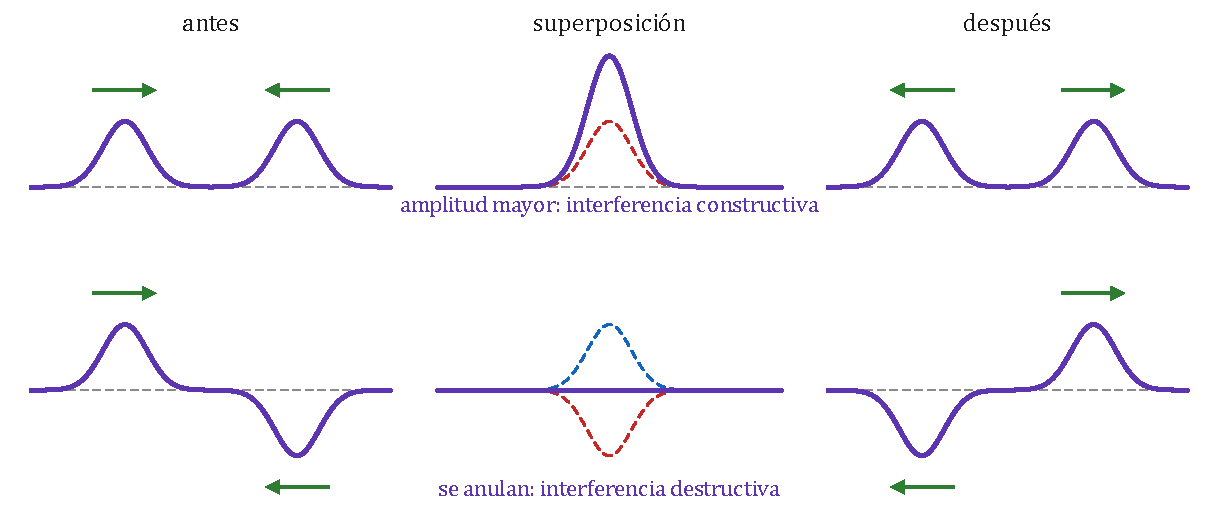
\includegraphics[width=0.9\linewidth]{images/UD2/interferencia_pulsos}
    \caption{Dos pulsos que se cruzan. Mientras coinciden, la forma de la cuerda es la suma de los dos (en discontinuo, cada
    pulso por separado). Después, cada uno sigue igual que antes.}
    \label{fig:ond-pulsos}
\end{figure}

\paragraph{Dos ondas de distinta amplitud.} Si en un punto coinciden dos m.a.s. de la misma frecuencia, con amplitudes
\(A_1\) y \(A_2\) y diferencia de fase \(\delta\), el resultado es otro m.a.s. de la misma frecuencia cuya amplitud se obtiene
sumando vectorialmente los dos \azuln{fasores} (vectores de módulo igual a la amplitud que giran con la fase):
\begin{centeredequation}
    A^2 = A_1^2 + A_2^2 + 2A_1A_2\cos\delta \label{eq:ond-fasores}
\end{centeredequation}
Si \(\delta = 2n\pi\), \(A = A_1 + A_2\) (máxima); si \(\delta = (2n - 1)\pi\), \(A = |A_1 - A_2|\) (mínima).

\subsection{Interferencia de dos ondas coherentes}\label{subsec:ond-coherentes}

Dos focos son \azuln{coherentes} si emiten ondas de la misma frecuencia con una diferencia de fase constante. Estudiaremos
el caso más sencillo: dos focos \(F_1\) y \(F_2\) que vibran en fase con la misma amplitud \(A\). A un punto \(P\) situado a
distancias \(x_1\) y \(x_2\) de los focos (figura~\ref{fig:ond-focos}) llegan:
\begin{equation*}
    y_1 = A\sen(\omega t - k x_1) \qquad\qquad y_2 = A\sen(\omega t - k x_2)
\end{equation*}

\begin{figure}[H]
    \centering
    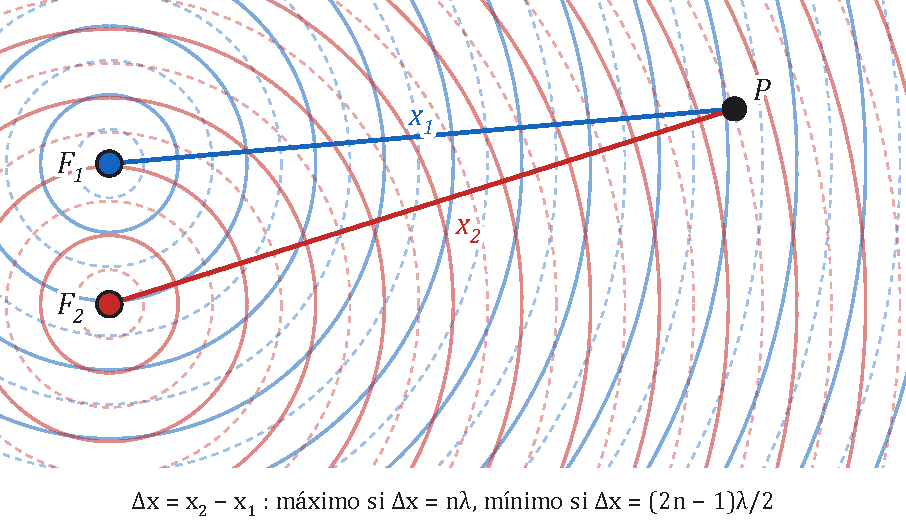
\includegraphics[width=0.6\linewidth]{images/UD2/interferencia_focos}
    \caption{Ondas emitidas por dos focos coherentes (crestas en línea continua y valles en discontinua). Lo que ocurre en
    \(P\) depende de la diferencia de caminos \(x_2 - x_1\).}
    \label{fig:ond-focos}
\end{figure}

Sumándolas con \(\sen a + \sen b = 2\sen\dfrac{a + b}{2}\cos\dfrac{a - b}{2}\):
\begin{centeredequation}
    y = \underbrace{2A\cos\left[\dfrac{k(x_2 - x_1)}{2}\right]}_{A_r}\,\sen\left[\omega t - k\,\dfrac{x_1 + x_2}{2}\right] \label{eq:ond-interferencia}
\end{centeredequation}
En \(P\) hay un m.a.s. de la misma frecuencia que las ondas, con una amplitud \(A_r\) que depende de la \textbf{diferencia de
caminos} \(\Delta x = x_2 - x_1\):
\begin{itemize}
    \item \textbf{Interferencia constructiva} (amplitud máxima, \(2A\)): \(\cos\dfrac{k\,\Delta x}{2} = \pm 1\), es decir,
    \[ \boxed{x_2 - x_1 = n\lambda} \qquad (n = 0, 1, 2\ldots) \]
    \item \textbf{Interferencia destructiva} (amplitud nula): \(\cos\dfrac{k\,\Delta x}{2} = 0\), es decir,
    \[ \boxed{x_2 - x_1 = (2n - 1)\,\dfrac{\lambda}{2}} \qquad (n = 1, 2, 3\ldots) \]
\end{itemize}

\begin{exercise}
    Dos altavoces conectados al mismo amplificador emiten en fase un sonido de \qty{680}{\hertz}
    (\(v = \qty{340}{\m\per\second}\)). ¿Qué tipo de interferencia hay en un punto que está a \qty{3}{\m} de un altavoz y a
    \qty{4.25}{\m} del otro? ¿Y en otro que está a \qty{3}{\m} y \qty{4}{\m}?
    \begin{solu}
        \textcolor{blue}{\(\lambda = \dfrac{v}{\nu} = \dfrac{340}{680} = \qty{0.5}{\m}\).}
        \begin{itemize}
            \item \(\Delta x = \qty{1.25}{\m} = 2{,}5\,\lambda = 5\cdot\dfrac{\lambda}{2}\): número impar de semilongitudes de onda,
            \textcolor{red}{interferencia destructiva} (apenas se oye).
            \item \(\Delta x = \qty{1}{\m} = 2\lambda\): \textcolor{red}{interferencia constructiva} (se oye más fuerte).
        \end{itemize}
    \end{solu}
\end{exercise}

\section{Ondas estacionarias}\label{sec:ond-estacionarias}

\begin{definition}[Onda estacionaria]
    Una \rojon{onda estacionaria} es el resultado de la interferencia de dos ondas iguales (misma amplitud, frecuencia y
    longitud de onda) que se propagan en la misma dirección y en sentidos contrarios.
\end{definition}

Es lo que ocurre en una cuerda sujeta por sus extremos, como la de una guitarra: las ondas se reflejan en los extremos y
las que van y las que vuelven se superponen.

\paragraph{Ecuación.} Tomemos el origen en el extremo fijo de una cuerda. La onda que llega viaja hacia las \(x\) negativas,
\(y_1 = A\sen(\omega t + kx)\). Al reflejarse en un extremo fijo cambia su fase en \(\pi\) (apartado~\ref{sec:ond-reflexion}),
así que la onda reflejada es \(y_2 = A\sen(\omega t - kx + \pi) = -A\sen(\omega t - kx)\). Sumando, con
\(\sen a - \sen b = 2\cos\dfrac{a + b}{2}\sen\dfrac{a - b}{2}\):
\begin{centeredequation}
    \boxed{y = 2A\sen(kx)\cos(\omega t)} \label{eq:ond-estacionaria}
\end{centeredequation}

Esta ecuación ya no tiene la forma \(\sen(\omega t \mp kx)\): no describe algo que avance. Cada punto vibra con un m.a.s. de
pulsación \(\omega\), pero con una amplitud que depende de su posición:
\begin{equation*}
    A_r = 2A\sen(kx)
\end{equation*}

\begin{itemize}
    \item \textbf{Nodos}: puntos que no vibran nunca (\(A_r = 0\)). \(\sen kx = 0 \Rightarrow kx = n\pi\):
    \[ \boxed{x = n\,\dfrac{\lambda}{2}} \qquad (n = 0, 1, 2\ldots) \]
    \item \textbf{Vientres} (o antinodos): puntos que vibran con la amplitud máxima, \(2A\). \(\sen kx = \pm 1 \Rightarrow
    kx = (2n - 1)\dfrac{\pi}{2}\):
    \[ \boxed{x = (2n - 1)\,\dfrac{\lambda}{4}} \qquad (n = 1, 2, 3\ldots) \]
\end{itemize}
Dos nodos (o dos vientres) consecutivos están separados \(\lambda/2\), y un nodo y el vientre siguiente, \(\lambda/4\)
(figura~\ref{fig:ond-estacionaria}).

\begin{figure}[H]
    \centering
    \begin{tikzpicture}
        \begin{axis}[fisica, width=0.8\linewidth, height=4.6cm, xmin=0, xmax=2.2, ymin=-1.5, ymax=1.6,
            xlabel={\(x\)}, ylabel={\(y\)}, xtick={0.5,1,1.5,2}, xticklabels={\(\frac{\lambda}{2}\),\(\lambda\),\(\frac{3\lambda}{2}\),\(2\lambda\)},
            ytick={-1,1}, yticklabels={\(-2A\),\(2A\)}]
            \pgfplotsinvokeforeach{0.5, -0.5, -1}{ \addplot[domain=0:2, thick, ocre!50, samples=120] {#1*sin(deg(2*pi*x))}; }
            \addplot[domain=0:2, very thick, ocre, samples=120] {sin(deg(2*pi*x))};
            \pgfplotsinvokeforeach{0, 0.5, 1, 1.5, 2}{ \node[circle, fill=blue, inner sep=1.6pt] at (axis cs:#1,0) {}; }
            \node[font=\small, blue, below] at (axis cs:0.5,-0.05) {N};
            \node[font=\small, red, above] at (axis cs:0.25,1.05) {V};
            \node[font=\small, red, above] at (axis cs:0.75,1.05) {V};
        \end{axis}
    \end{tikzpicture}
    \caption{Onda estacionaria en varios instantes. Los nodos (N) están siempre quietos; los vientres (V) oscilan con la
    amplitud máxima. Todos los puntos entre dos nodos vibran en fase.}
    \label{fig:ond-estacionaria}
\end{figure}

\begin{remark}
    Una onda estacionaria \textbf{no transporta energía} de un sitio a otro: la energía queda «atrapada» entre los nodos.
    No es, en sentido estricto, un movimiento ondulatorio, sino una forma de vibrar de todo el medio.
\end{remark}

Si las dos ondas que se superponen son \(y_1 = A\sen(\omega t + kx)\) e \(y_2 = A\sen(\omega t - kx)\) (sin el cambio de
fase), se obtiene \(y = 2A\cos(kx)\sen(\omega t)\). En ese caso los papeles se intercambian: hay un vientre en \(x = 0\), los
vientres están en \(x = n\lambda/2\) y los nodos en \(x = (2n - 1)\lambda/4\). Esta forma aparece, por ejemplo, en el
extremo abierto de un tubo.

\begin{exercise}
    Una cuerda vibra según la ecuación \(y = 4\sen\left(\dfrac{\pi}{4}x\right)\cos(30\pi t)\), con \(x\) e \(y\) en
    centímetros y \(t\) en segundos. Calcula:
    \begin{enumerate}[label=\letraminuscula]
        \item La amplitud y la velocidad de las ondas que la forman.
        \item La velocidad de vibración del punto \(x = \qty{1}{\cm}\) en \(t = \qty{0.05}{\second}\).
        \item La amplitud de un vientre y la distancia entre dos nodos consecutivos.
        \item La distancia entre el primer nodo (\(x = 0\)) y el tercer vientre.
    \end{enumerate}
    \begin{solu}
        \textcolor{blue}{Comparando con \(y = 2A\sen(kx)\cos(\omega t)\): \(2A = \qty{4}{\cm}\), \(k = \dfrac{\pi}{4}\ \unit{\per\cm}\), \(\omega = 30\pi\ \unit{\radian\per\second}\).}
        \begin{enumerate}[label=\letraminuscula]
            \item \(A = \textcolor{red}{\qty{2}{\cm}}\). \(\lambda = \dfrac{2\pi}{k} = \qty{8}{\cm}\), \(\nu = \dfrac{\omega}{2\pi} = \qty{15}{\hertz}\):
            \(v = \lambda\nu = \textcolor{red}{\qty{120}{\cm\per\second} = \qty{1.2}{\m\per\second}}\).
            \item \(v_y = \dfrac{\partial y}{\partial t} = -4\cdot 30\pi\sen\left(\dfrac{\pi}{4}x\right)\sen(30\pi t)\).
            Con \(x = 1\), \(t = 0{,}05\): \(v_y = -120\pi\cdot\sen\dfrac{\pi}{4}\cdot\sen\dfrac{3\pi}{2} = \textcolor{red}{\qty{267}{\cm\per\second}}\).
            \item Vientre: \(2A = \textcolor{red}{\qty{4}{\cm}}\). Entre nodos: \(\dfrac{\lambda}{2} = \textcolor{red}{\qty{4}{\cm}}\).
            \item \textcolor{blue}{Los vientres están en \(x = (2n - 1)\lambda/4 = 2, 6, 10\ldots\) cm.} El tercero está a \textcolor{red}{\qty{10}{\cm}} del primer nodo.
        \end{enumerate}
    \end{solu}
\end{exercise}

\begin{exercise}
    Para la onda estacionaria \(y = 2A\cos(kx)\sen(\omega t)\), deduce dónde están los vientres y los nodos y la distancia
    entre dos nodos consecutivos.
    \begin{solu}
        \textcolor{blue}{La amplitud es \(A_r = 2A\cos kx\).}
        \begin{itemize}
            \item Vientres: \(\cos kx = \pm 1 \Rightarrow kx = n\pi \Rightarrow \textcolor{red}{x = n\,\dfrac{\lambda}{2}}\) (\(n = 0, 1, 2\ldots\)).
            \item Nodos: \(\cos kx = 0 \Rightarrow kx = (2n - 1)\dfrac{\pi}{2} \Rightarrow \textcolor{red}{x = (2n - 1)\,\dfrac{\lambda}{4}}\).
            \item Entre nodos consecutivos: \(\dfrac{3\lambda}{4} - \dfrac{\lambda}{4} = \textcolor{red}{\dfrac{\lambda}{2}}\), igual que antes.
        \end{itemize}
    \end{solu}
\end{exercise}

\subsection{Armónicos}\label{subsec:ond-armonicos}

En una cuerda de longitud \(L\) no se puede formar cualquier onda estacionaria: los extremos imponen condiciones
(figura~\ref{fig:ond-armonicos}).

\paragraph{Cuerda con los dos extremos fijos} (guitarra, piano, violín). Los dos extremos tienen que ser nodos, así que en
la cuerda debe caber un número entero de semilongitudes de onda:
\begin{equation*}
    L = n\,\dfrac{\lambda}{2} \;\Rightarrow\; \lambda_n = \dfrac{2L}{n} \;\Rightarrow\; \boxed{\nu_n = \dfrac{v}{\lambda_n} = n\,\dfrac{v}{2L} = n\,\nu_1} \qquad (n = 1, 2, 3\ldots)
\end{equation*}
La frecuencia más baja, \(\nu_1 = v/2L\), es la \azuln{frecuencia fundamental} (o primer armónico). Las demás son múltiplos
enteros de ella: son los \azuln{armónicos}.

\paragraph{Cuerda con un extremo fijo y otro libre} (y también un tubo cerrado por un extremo). El extremo fijo es un nodo y
el libre es un vientre, así que la longitud debe ser un número impar de cuartos de longitud de onda:
\begin{equation*}
    L = (2n - 1)\,\dfrac{\lambda}{4} \;\Rightarrow\; \lambda = \dfrac{4L}{2n - 1} \;\Rightarrow\; \boxed{\nu = (2n - 1)\,\dfrac{v}{4L}} \qquad (n = 1, 2, 3\ldots)
\end{equation*}
Solo aparecen los armónicos \textbf{impares} de la fundamental \(\nu_1 = v/4L\): el tercero (\(n = 2\)), el quinto (\(n = 3\))\ldots

\begin{figure}[H]
    \centering
    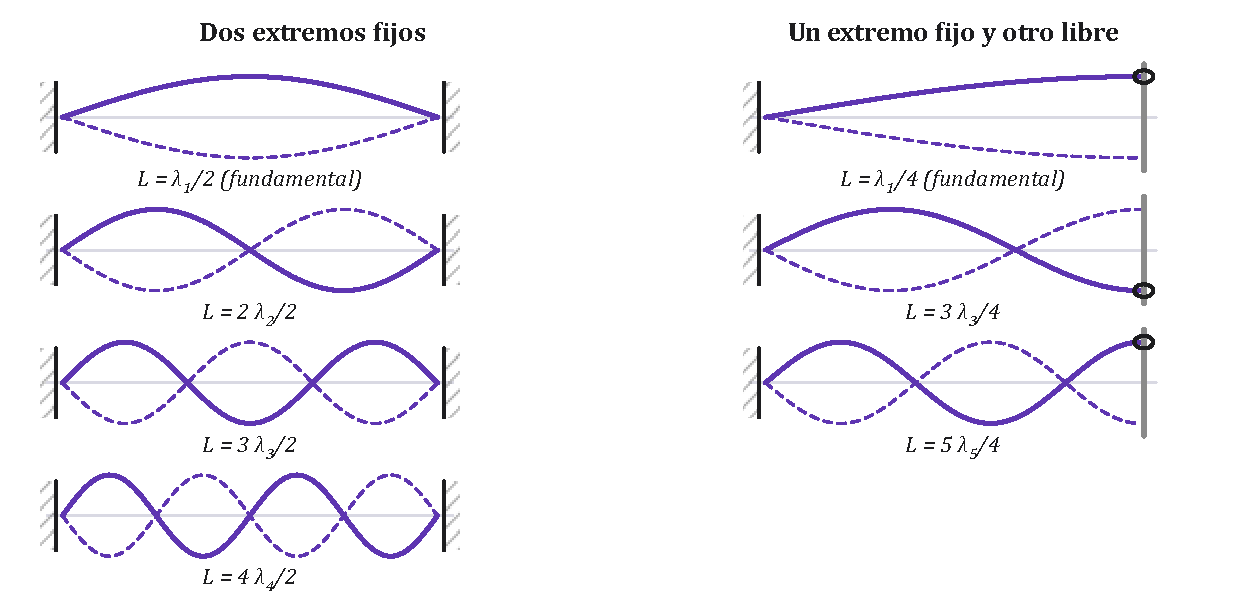
\includegraphics[width=0.95\linewidth]{images/UD2/armonicos}
    \caption{Modos de vibración de una cuerda de longitud \(L\). Con los dos extremos fijos caben \(n\) husos de longitud
    \(\lambda/2\); con un extremo libre, un número impar de cuartos de onda.}
    \label{fig:ond-armonicos}
\end{figure}

\begin{exercise}
    La cuerda La de una guitarra mide \qty{65}{\cm} entre sus dos apoyos y su frecuencia fundamental es \qty{110}{\hertz}.
    Calcula la velocidad de las ondas en la cuerda y las frecuencias de sus dos armónicos siguientes.
    \begin{solu}
        \textcolor{blue}{Fundamental: \(\lambda_1 = 2L = \qty{1.30}{\m}\).} \(v = \lambda_1\nu_1 = 1{,}30\cdot 110 = \textcolor{red}{\qty{143}{\m\per\second}}\).

        \(\nu_2 = 2\nu_1 = \textcolor{red}{\qty{220}{\hertz}}\); \(\nu_3 = 3\nu_1 = \textcolor{red}{\qty{330}{\hertz}}\).
        \textcolor{blue}{(Al pisar un traste se acorta \(L\) y sube la frecuencia.)}
    \end{solu}
\end{exercise}

\section{Principio de Huygens}\label{sec:ond-huygens}

En 1678 Christiaan Huygens propuso un método geométrico para saber cómo avanza un frente de onda. Cuando la onda alcanza un
punto, éste empieza a vibrar y se comporta como un nuevo foco que emite pequeñas ondas, las \azuln{ondas secundarias}.

\begin{definition}[Principio de Huygens]
    Cada punto de un frente de onda se comporta como un foco de ondas secundarias. Al cabo de un tiempo, el nuevo frente de
    onda es la superficie tangente a todas esas ondas secundarias (su \azuln{envolvente}).
\end{definition}

\begin{figure}[H]
    \centering
    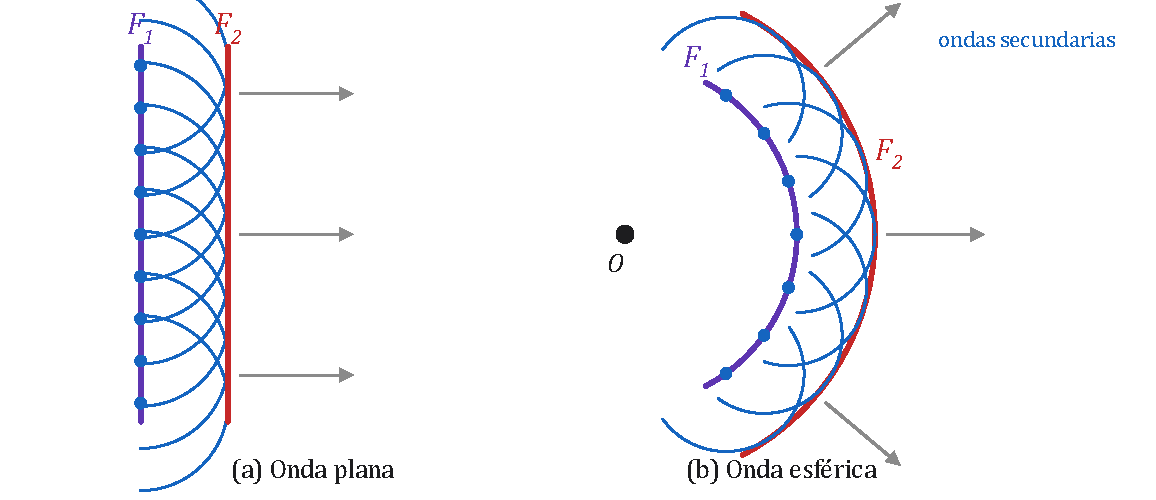
\includegraphics[width=0.85\linewidth]{images/UD2/huygens}
    \caption{Construcción de Huygens. Los puntos del frente \(F_1\) emiten ondas secundarias; su envolvente es el frente
    \(F_2\). Con este principio se explican la difracción, la reflexión y la refracción.}
    \label{fig:ond-huygens}
\end{figure}

\section{Difracción}\label{sec:ond-difraccion}

\begin{definition}[Difracción]
    La \rojon{difracción} es la desviación que sufre una onda al encontrar un obstáculo o una abertura: la onda lo rodea y
    se propaga también por detrás. Es apreciable cuando el tamaño del obstáculo o de la abertura es \textbf{parecido a la
    longitud de onda}.
\end{definition}

Según el principio de Huygens, los puntos de la abertura que la onda alcanza se convierten en focos de ondas secundarias
que se propagan en todas direcciones detrás de la pared. Si la abertura es mucho mayor que \(\lambda\), solo se curvan los
bordes del frente y la onda pasa casi sin cambios; si es del orden de \(\lambda\), la abertura se comporta como un foco
puntual y la onda se abre en semicircunferencias (figura~\ref{fig:ond-difraccion}).

\begin{figure}[H]
    \centering
    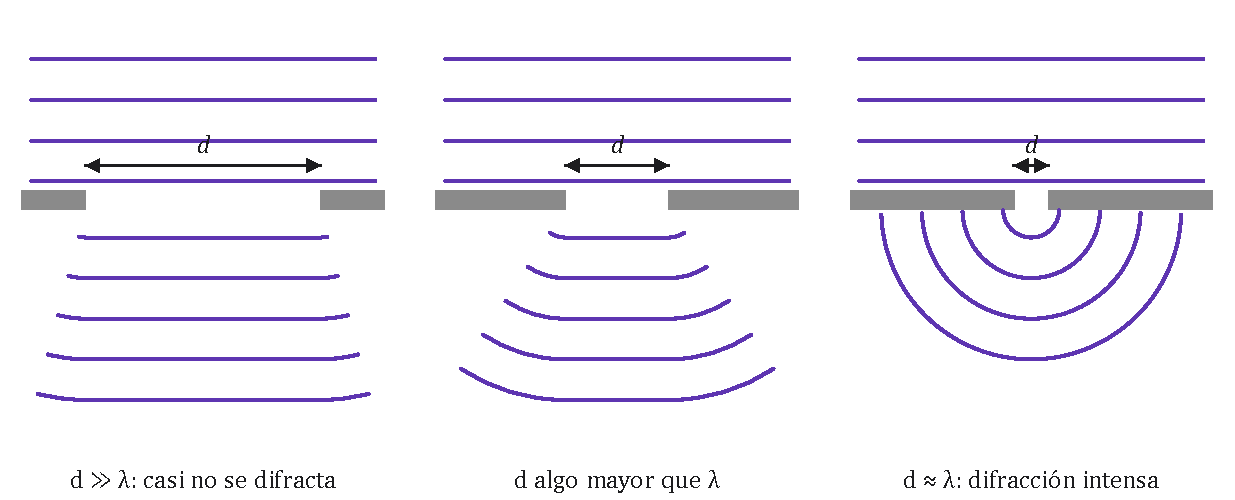
\includegraphics[width=0.95\linewidth]{images/UD2/difraccion}
    \caption{Ondas planas que llegan a una abertura de anchura \(d\). Cuanto más se parece \(d\) a la longitud de onda,
    más se difracta la onda.}
    \label{fig:ond-difraccion}
\end{figure}

La difracción es la razón de que oigamos a alguien que habla detrás de una esquina: las longitudes de onda del sonido (de
centímetros a metros) son parecidas al tamaño de puertas y edificios. La luz, con \(\lambda\) de unos \qty{500}{\nm}, solo
se difracta apreciablemente en rendijas muy estrechas; por eso la difracción es la prueba de que algo se comporta como una
onda.

\section{Reflexión}\label{sec:ond-reflexion}

\begin{definition}[Reflexión]
    La \rojon{reflexión} es el cambio de dirección que sufre una onda al chocar con la superficie de separación con otro
    medio, de forma que vuelve al medio de donde venía. Como no cambia de medio, \textbf{su velocidad, su frecuencia y su
    longitud de onda no cambian}.
\end{definition}

Para describirla se usa la \azuln{normal}, la recta perpendicular a la superficie en el punto de incidencia. El
\azuln{ángulo de incidencia} \(\hat{\imath}\) es el que forma el rayo incidente con la normal, y el \azuln{ángulo de
reflexión} \(\hat r\), el que forma el rayo reflejado con la normal (figura~\ref{fig:ond-reflexion}).

\begin{figure}[H]
    \centering
    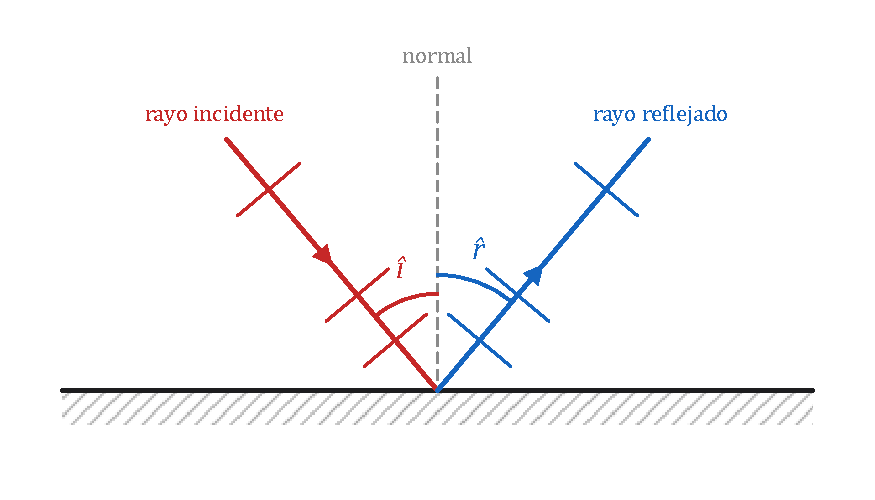
\includegraphics[width=0.52\linewidth]{images/UD2/reflexion}
    \caption{Reflexión de una onda plana. Los segmentos cortos representan los frentes de onda.}
    \label{fig:ond-reflexion}
\end{figure}

\paragraph{Leyes de la reflexión.}
\begin{enumerate}[label=\numberballmDarkTeal]
    \item El rayo incidente, la normal y el rayo reflejado están en el mismo plano.
    \item El ángulo de incidencia es igual al de reflexión: \(\boxed{\hat{\imath} = \hat r}\).
\end{enumerate}
Se deducen con el principio de Huygens: mientras un extremo del frente incidente recorre la distancia que le falta hasta la
superficie, la onda secundaria emitida por el otro extremo recorre la misma distancia en el mismo medio. Los dos triángulos
rectángulos que se forman son iguales y, por tanto, también los ángulos.

\paragraph{Cambio de fase en la reflexión.} Cuando un pulso que viaja por una cuerda llega a un \textbf{extremo fijo}, la
cuerda tira del soporte y, por la tercera ley de Newton, el soporte tira de la cuerda en sentido contrario: el pulso vuelve
\textbf{invertido}, con un cambio de fase de \(\pi\). Si el extremo es \textbf{libre} (por ejemplo, una anilla que desliza
sin rozamiento por una varilla), el pulso vuelve \textbf{sin invertirse} (figura~\ref{fig:ond-reflexion-pulso}).

\begin{figure}[H]
    \centering
    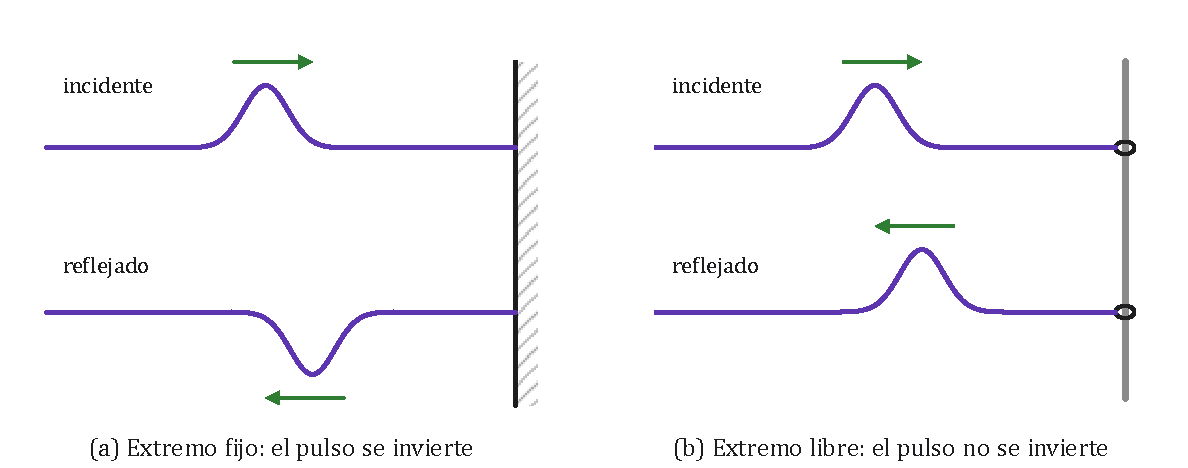
\includegraphics[width=0.88\linewidth]{images/UD2/reflexion_pulso}
    \caption{Reflexión de un pulso en el extremo de una cuerda.}
    \label{fig:ond-reflexion-pulso}
\end{figure}

\section{Refracción}\label{sec:ond-refraccion}

\begin{definition}[Refracción]
    La \rojon{refracción} es el cambio de dirección que sufre una onda al pasar de un medio a otro en el que su velocidad de
    propagación es distinta. La \textbf{frecuencia no cambia} (la impone el foco), pero sí la velocidad y, por tanto, la
    longitud de onda.
\end{definition}

\paragraph{Leyes de la refracción.}
\begin{enumerate}[label=\numberballmDarkTeal]
    \item El rayo incidente, la normal y el rayo refractado están en el mismo plano.
    \item El ángulo de incidencia y el de refracción cumplen la \rojon{ley de Snell}:
    \begin{centeredequation}
        \boxed{\dfrac{\sen\hat{\imath}}{\sen\hat r} = \dfrac{v_1}{v_2}} \label{eq:ond-snell}
    \end{centeredequation}
\end{enumerate}

\begin{figure}[H]
    \centering
    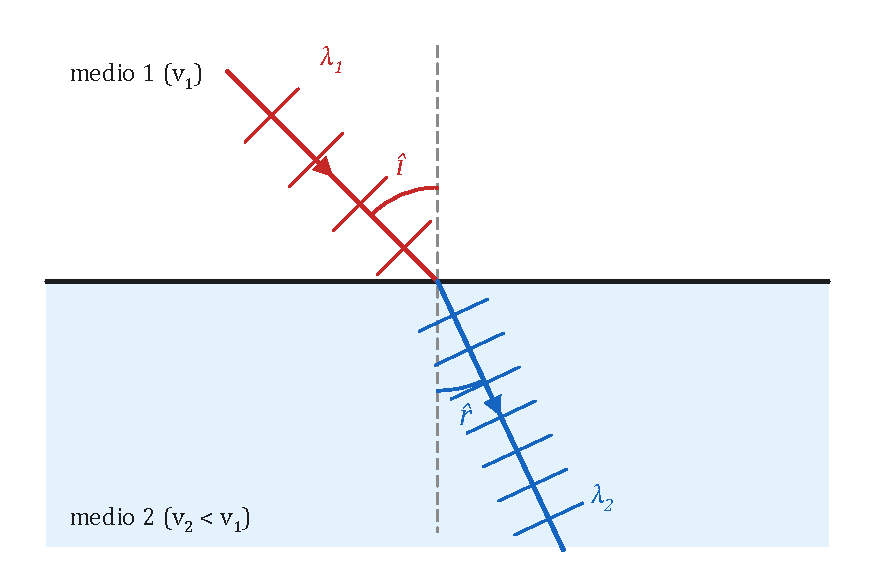
\includegraphics[width=0.52\linewidth]{images/UD2/refraccion}
    \caption{Al entrar en un medio donde va más despacio, la onda se acerca a la normal y sus frentes se juntan
    (\(\lambda_2 < \lambda_1\)).}
    \label{fig:ond-refraccion}
\end{figure}

\paragraph{Deducción con el principio de Huygens.} Un frente plano llega oblicuamente a la superficie. Su extremo \(A\)
toca primero la superficie y emite una onda secundaria hacia el medio 2. En el tiempo \(t\) que tarda el otro extremo en
llegar a la superficie (recorriendo \(v_1 t\)), la onda secundaria de \(A\) avanza \(v_2 t\) en el medio 2. Si \(d\) es la
distancia sobre la superficie entre los dos puntos de llegada, la geometría da \(v_1 t = d\sen\hat{\imath}\) y
\(v_2 t = d\sen\hat r\). Dividiendo, se obtiene la ley de Snell. Si \(v_2 < v_1\), el rayo se acerca a la normal; si
\(v_2 > v_1\), se aleja.

\begin{remark}
    En la reflexión la onda no cambia de medio, \(v_1 = v_2\), y la ley de Snell da \(\sen\hat{\imath} = \sen\hat r\), es
    decir, \(\hat{\imath} = \hat r\): la segunda ley de la reflexión.
\end{remark}

\begin{exercise}
    Un sonido pasa del aire (\qty{340}{\m\per\second}) al agua (\qty{1450}{\m\per\second}) con un ángulo de incidencia de
    \ang{10}. ¿Con qué ángulo se refracta? ¿Qué ocurre si el ángulo de incidencia es mayor de \ang{13.6}?
    \begin{solu}
        \(\sen\hat r = \dfrac{v_2}{v_1}\sen\hat{\imath} = \dfrac{1450}{340}\sen\ang{10} = 0{,}741 \Rightarrow \textcolor{red}{\hat r = \ang{47.8}}\):
        \textcolor{blue}{se aleja mucho de la normal porque en el agua va más deprisa.}

        \textcolor{blue}{El ángulo de refracción llega a \ang{90} cuando \(\sen\hat{\imath} = \dfrac{340}{1450} = 0{,}234\), es decir, \(\hat{\imath} = \ang{13.6}\).}
        \textcolor{red}{Para ángulos mayores no hay onda refractada: el sonido se refleja por completo} \textcolor{blue}{(reflexión total, que estudiaremos en óptica).}
    \end{solu}
\end{exercise}

\section{Polarización}\label{sec:ond-polarizacion}

En una onda transversal que avanza en la dirección del eje \(X\), cada punto puede vibrar en cualquier dirección del plano
\(YZ\). Si la vibración se produce siempre en una misma dirección, decimos que la onda está \rojon{polarizada linealmente}.

Si agitamos de arriba abajo una cuerda que pasa por una rendija vertical, la onda la atraviesa; si la rendija es
horizontal, la onda no pasa (figura~\ref{fig:ond-polarizacion}). Una rendija así actúa como un \azuln{polarizador}: solo
deja pasar la vibración en una dirección.

\begin{figure}[H]
    \centering
    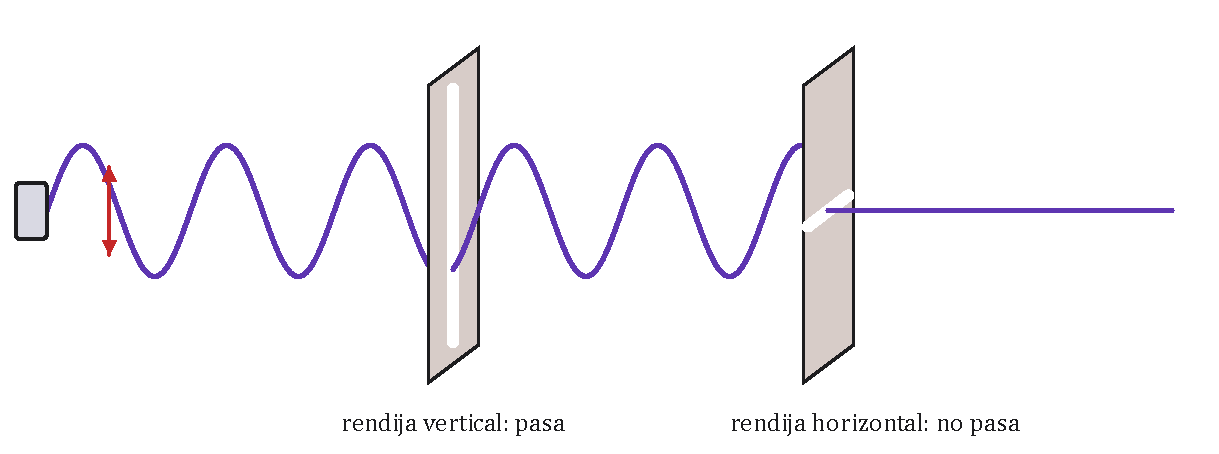
\includegraphics[width=0.9\linewidth]{images/UD2/polarizacion}
    \caption{Una onda que vibra en vertical atraviesa una rendija vertical, pero una rendija horizontal la detiene.}
    \label{fig:ond-polarizacion}
\end{figure}

\begin{remark}
    \textbf{Solo se pueden polarizar las ondas transversales}: en una onda longitudinal la vibración tiene la dirección de
    la propagación y cualquier rendija la deja pasar. Por eso la luz se puede polarizar (es transversal) y el sonido no.
    Las gafas de sol polarizadas y las pantallas LCD aprovechan este fenómeno.
\end{remark}

\section{Efecto Doppler}\label{sec:ond-doppler}

Cuando una ambulancia se acerca, su sirena suena más aguda, y al alejarse, más grave. El \rojon{efecto Doppler} es el
cambio de la frecuencia percibida por un observador cuando el foco, el observador o ambos se mueven el uno respecto del
otro. Llamemos \(\nu\) a la frecuencia emitida, \(\nu'\) a la percibida, \(v\) a la velocidad del sonido,
\(v_O\) a la del observador y \(v_F\) a la del foco.

\paragraph{Observador en movimiento, foco quieto.} Si el observador se acerca al foco, encuentra las ondas a una velocidad
relativa \(v + v_O\). La longitud de onda no cambia, \(\lambda = v/\nu\), así que le llegan más frentes por segundo:
\begin{equation*}
    \nu' = \dfrac{v + v_O}{\lambda} = \nu\,\dfrac{v + v_O}{v} \qquad \text{(si se aleja: } v - v_O\text{)}
\end{equation*}

\paragraph{Foco en movimiento, observador quieto.} Ahora los frentes no son concéntricos: el foco «persigue» a las ondas
que emite hacia delante (figura~\ref{fig:ond-doppler}). Mientras un frente avanza \(\lambda = vT\), el foco avanza
\(v_F T\), y la distancia entre frentes delante del foco es \(\lambda' = (v - v_F)\,T\). El observador que tiene delante
percibe:
\begin{equation*}
    \nu' = \dfrac{v}{\lambda'} = \nu\,\dfrac{v}{v - v_F} \qquad \text{(si el foco se aleja: } v + v_F\text{)}
\end{equation*}

\begin{figure}[H]
    \centering
    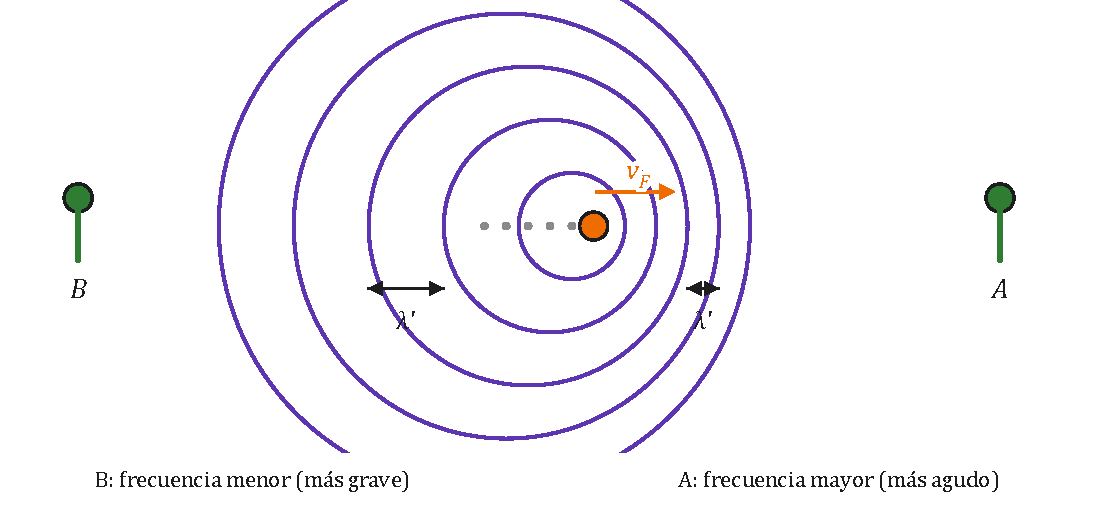
\includegraphics[width=0.72\linewidth]{images/UD2/doppler}
    \caption{Frentes de onda emitidos por un foco que se mueve hacia la derecha. El observador \(A\) recibe los frentes más
    juntos (frecuencia mayor) y el \(B\), más separados (frecuencia menor).}
    \label{fig:ond-doppler}
\end{figure}

\paragraph{Caso general.} Juntando los dos efectos:
\begin{centeredequation}
    \boxed{\nu' = \nu\,\dfrac{v \pm v_O}{v \mp v_F}} \label{eq:ond-doppler}
\end{centeredequation}
\begin{itemize}
    \item Se usan los \textbf{signos de arriba} (\(+v_O\) en el numerador, \(-v_F\) en el denominador) cuando el observador o
    el foco se mueven \textbf{acercándose} al otro.
    \item Se usan los \textbf{signos de abajo} cuando se mueven \textbf{alejándose}.
\end{itemize}
Comprobación rápida: al acercarse, la frecuencia percibida debe salir \emph{mayor} que la emitida; al alejarse, menor.

\begin{exercise}
    Una ambulancia circula a \qty{90}{\km\per\hour} con la sirena encendida a \qty{700}{\hertz}. ¿Qué frecuencia oye un
    peatón parado cuando la ambulancia se acerca? ¿Y cuando se aleja? (\(v = \qty{340}{\m\per\second}\)).
    \begin{solu}
        \textcolor{blue}{\(v_F = \qty{25}{\m\per\second}\), \(v_O = 0\).}

        Se acerca: \(\nu' = 700\cdot\dfrac{340}{340 - 25} = \textcolor{red}{\qty{756}{\hertz}}\).
        Se aleja: \(\nu' = 700\cdot\dfrac{340}{340 + 25} = \textcolor{red}{\qty{652}{\hertz}}\).

        \textcolor{blue}{Al pasar a su lado, el peatón oye bajar el tono unos \qty{100}{\hertz}.}
    \end{solu}
\end{exercise}

\begin{exercise}
    Un coche patrulla circula a \qty{108}{\km\per\hour} con la sirena a \qty{600}{\hertz} y se acerca a un ciclista que va
    hacia él a \qty{72}{\km\per\hour}. ¿Qué frecuencia oye el ciclista? ¿Y después de cruzarse?
    \begin{solu}
        \textcolor{blue}{\(v_F = \qty{30}{\m\per\second}\), \(v_O = \qty{20}{\m\per\second}\). Antes de cruzarse, los dos se acercan:}
        \(\nu' = 600\cdot\dfrac{340 + 20}{340 - 30} = \textcolor{red}{\qty{697}{\hertz}}\).

        \textcolor{blue}{Después, los dos se alejan:} \(\nu' = 600\cdot\dfrac{340 - 20}{340 + 30} = \textcolor{red}{\qty{519}{\hertz}}\).
    \end{solu}
\end{exercise}

\begin{remark}
    El efecto Doppler tiene muchas aplicaciones: los radares de tráfico miden la velocidad de los coches con el cambio de
    frecuencia de las ondas que rebotan en ellos; las ecografías Doppler miden la velocidad de la sangre; y en astronomía
    el desplazamiento de la luz de las galaxias hacia el rojo indica que se alejan de nosotros (expansión del universo).
\end{remark}

\section{Resumen de fórmulas}\label{sec:ond-resumen}

\begin{table}[H]
    \centering
    \caption{Fórmulas principales del movimiento ondulatorio}
    \vspace{-5pt}
    \begin{tabular}{@{}lL{10cm}@{}}
        \toprule
        \textbf{Magnitud} & \textbf{Expresión} \\
        \midrule
        Relaciones básicas & \(\lambda = vT = v/\nu\), \quad \(k = 2\pi/\lambda\), \quad \(\omega = 2\pi\nu\), \quad \(v = \omega/k\) \\[3pt]
        Ecuación de onda & \(y = A\sen(\omega t \mp kx + \varphi_0)\) \quad (\(-\): hacia \(+X\); \(+\): hacia \(-X\)) \\[3pt]
        Velocidad de vibración & \(v_y = A\omega\cos(\omega t - kx + \varphi_0)\), \quad \(v_{y,\text{máx}} = A\omega\) \\[3pt]
        Puntos en fase / oposición & \(\Delta x = n\lambda\) \quad / \quad \(\Delta x = (2n - 1)\lambda/2\) \\[3pt]
        Intensidad & \(I = P/S\), \quad \(I = P/(4\pi r^2)\), \quad \(I_1/I_2 = r_2^2/r_1^2 = A_1^2/A_2^2\) \\[3pt]
        Absorción & \(I = I_0\,e^{-\beta x}\) \\[3pt]
        Nivel de intensidad sonora & \(\beta = 10\log(I/I_0)\), \quad \(I_0 = \qty{e-12}{\watt\per\square\m}\) \\[3pt]
        Interferencia (focos en fase) & máximo: \(x_2 - x_1 = n\lambda\); \quad mínimo: \(x_2 - x_1 = (2n - 1)\lambda/2\) \\[3pt]
        Onda estacionaria & \(y = 2A\sen(kx)\cos(\omega t)\) \\[3pt]
        Nodos y vientres & nodos en \(x = n\lambda/2\); \quad vientres en \(x = (2n - 1)\lambda/4\) \\[3pt]
        Armónicos & dos extremos fijos: \(\nu_n = n\,v/2L\); \quad un extremo libre: \(\nu = (2n - 1)\,v/4L\) \\[3pt]
        Ley de Snell & \(\sen\hat{\imath}/\sen\hat r = v_1/v_2\) \\[3pt]
        Efecto Doppler & \(\nu' = \nu\,(v \pm v_O)/(v \mp v_F)\) \quad (signos de arriba: acercándose) \\
        \bottomrule
    \end{tabular}
    \label{tab:ond-resumen}
\end{table}

\section{Prácticas de laboratorio}\label{sec:ond-practicas}

\subsection{Práctica 1: ondas estacionarias en una cuerda}\label{subsec:ond-practica-melde}

\noindent\begin{minipage}[t]{0.58\linewidth}
\textbf{Objetivo.} Producir ondas estacionarias en una cuerda (experiencia de Melde), comprobar que solo aparecen ciertos
modos de vibración y medir la velocidad de las ondas.

\textbf{Material.} Vibrador de frecuencia conocida (o generador de funciones con un excitador), cuerda o hilo elástico,
polea con soporte, portapesas y pesas, regla, balanza.

\textbf{Procedimiento.}
\begin{enumerate}[label=\numberballmDarkTeal]
    \item Mide la masa y la longitud de un trozo largo de cuerda para calcular \(\mu = m/l\).
    \item Monta el dispositivo de la figura~\ref{fig:ond-practica-melde}: la cuerda va del vibrador a la polea y del otro
    extremo cuelgan las pesas. La tensión es \(T = m g\).
    \item Enciende el vibrador y cambia la masa colgada (o la frecuencia) hasta que se vea una onda estacionaria nítida.
    Cuenta los husos \(n\) y mide la longitud \(L\) entre el vibrador y la polea.
    \item Repite para varios valores de \(n\).
\end{enumerate}
\end{minipage}\hfill
\begin{minipage}[t]{0.38\linewidth}
    \vspace{0pt}
    \centering
    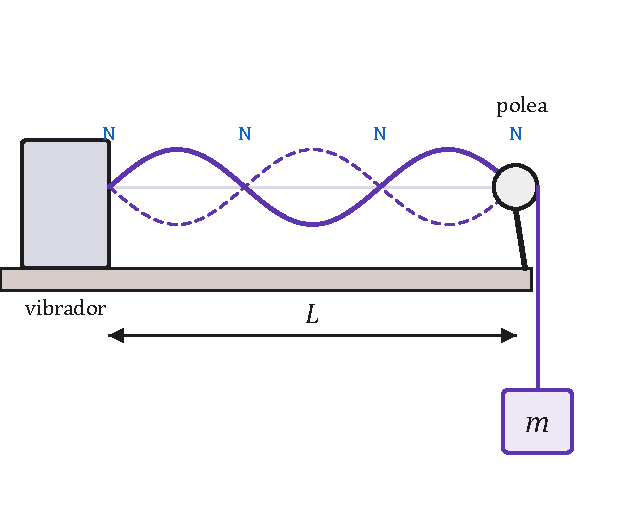
\includegraphics[width=\linewidth]{images/UD2/practica_melde}
    \captionof{figure}{Montaje de la experiencia de Melde.}
    \label{fig:ond-practica-melde}
\end{minipage}

\begin{table}[H]
    \centering
    \caption{Datos de la práctica de ondas estacionarias}
    \vspace{-5pt}
    \begin{tabular}{@{}C{2cm}C{1.6cm}C{2cm}C{2.4cm}C{2.4cm}C{2.4cm}@{}}
        \toprule
        \textbf{\(m\) (\unit{\kg})} & \textbf{\(n\)} & \textbf{\(L\) (\unit{\m})} & \textbf{\(\lambda = 2L/n\) (\unit{\m})} & \textbf{\(v = \lambda\nu\) (\unit{\m\per\second})} & \textbf{\(v = \sqrt{T/\mu}\) (\unit{\m\per\second})} \\
        \midrule
        \rule{0pt}{18pt} & & & & & \\ \midrule[0.3pt]
        \rule{0pt}{18pt} & & & & & \\ \midrule[0.3pt]
        \rule{0pt}{18pt} & & & & & \\
        \bottomrule
    \end{tabular}
    \label{tab:ond-practica-melde}
\end{table}

\textbf{Cálculos.} Con los dos extremos fijos (el vibrador y la polea son casi nodos), \(\lambda = 2L/n\) y
\(v = \lambda\nu\). Compara ese valor con el teórico \(v = \sqrt{T/\mu}\).

\textbf{Cuestiones.}
\begin{enumerate}[label=\letraminuscula]
    \item Si con una masa de \qty{200}{\g} y \(\mu = \qty{2}{\g\per\m}\) la velocidad teórica es \qty{31.3}{\m\per\second},
    ¿cuántos husos esperas ver con \(\nu = \qty{50}{\hertz}\) y \(L = \qty{1.25}{\m}\)?
    \item ¿Qué le pasa al número de husos si aumentas la masa colgada? Explícalo.
    \item ¿Por qué entre dos modos de vibración la cuerda apenas se mueve?
\end{enumerate}

\subsection{Práctica 2: velocidad del sonido con un tubo de resonancia}\label{subsec:ond-practica-tubo}

\noindent\begin{minipage}[t]{0.64\linewidth}
\textbf{Objetivo.} Medir la velocidad del sonido en el aire usando la resonancia de una columna de aire.

\textbf{Material.} Tubo de vidrio o de plástico de \qty{1}{\m} aproximadamente, probeta alta o recipiente con agua (para
variar el nivel), diapasones de frecuencia conocida (o una aplicación de móvil que emita un tono puro), regla y termómetro.

\textbf{Fundamento.} El tubo, cerrado abajo por el agua, se comporta como una cuerda con un extremo fijo y otro libre: en
la superficie del agua hay un nodo y en la boca del tubo, un vientre. La primera resonancia se produce cuando la columna de
aire mide \(L_1 = \lambda/4\) y la segunda cuando mide \(L_2 = 3\lambda/4\); entre las dos hay \(\lambda/2\).

\textbf{Procedimiento.}
\begin{enumerate}[label=\numberballmDarkTeal]
    \item Golpea el diapasón y sostenlo sobre la boca del tubo (figura~\ref{fig:ond-practica-tubo}).
    \item Sube o baja el tubo (o el nivel del agua) hasta que el sonido se refuerce claramente. Mide \(L_1\).
    \item Sigue alargando la columna de aire hasta la siguiente resonancia y mide \(L_2\).
    \item Repite con otros diapasones y anota la temperatura del laboratorio.
\end{enumerate}
\end{minipage}\hfill
\begin{minipage}[t]{0.32\linewidth}
    \vspace{0pt}
    \centering
    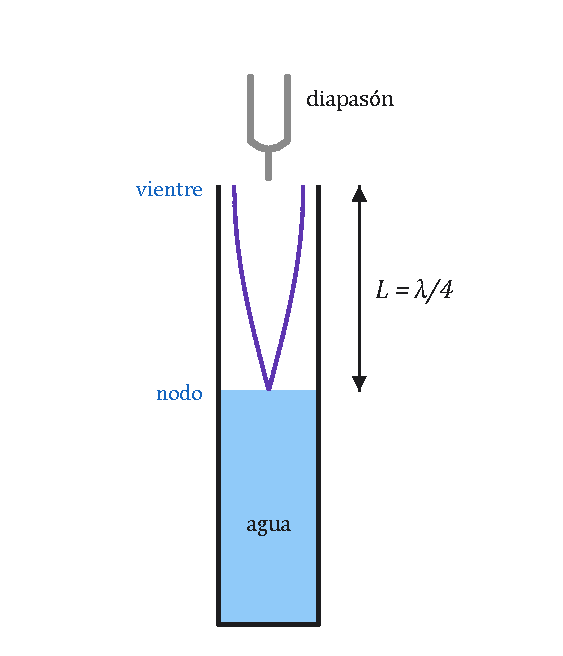
\includegraphics[width=0.85\linewidth]{images/UD2/practica_tubo}
    \captionof{figure}{Columna de aire en resonancia.}
    \label{fig:ond-practica-tubo}
\end{minipage}

\begin{table}[H]
    \centering
    \caption{Datos de la práctica del tubo de resonancia}
    \vspace{-5pt}
    \begin{tabular}{@{}C{2.2cm}C{2.2cm}C{2.2cm}C{3.2cm}C{3cm}@{}}
        \toprule
        \textbf{\(\nu\) (\unit{\hertz})} & \textbf{\(L_1\) (\unit{\m})} & \textbf{\(L_2\) (\unit{\m})} & \textbf{\(\lambda = 2(L_2 - L_1)\) (\unit{\m})} & \textbf{\(v = \lambda\nu\) (\unit{\m\per\second})} \\
        \midrule
        \rule{0pt}{18pt} & & & & \\ \midrule[0.3pt]
        \rule{0pt}{18pt} & & & & \\ \midrule[0.3pt]
        \rule{0pt}{18pt} & & & & \\
        \bottomrule
    \end{tabular}
    \label{tab:ond-practica-tubo}
\end{table}

\textbf{Cálculos.} Usa \(\lambda = 2(L_2 - L_1)\): así no influye que el vientre esté en realidad un poco por encima de la
boca del tubo. Calcula \(v = \lambda\nu\) y su valor medio.

\textbf{Cuestiones.}
\begin{enumerate}[label=\letraminuscula]
    \item Compara tu resultado con el teórico \(v = \sqrt{\gamma R T/M}\) a la temperatura del laboratorio
    (\(\gamma = 1{,}4\); \(M = \qty{0.029}{\kg\per\mol}\)) y calcula el error relativo.
    \item Calcula \(4L_1\) y compáralo con \(\lambda\). ¿Por qué no coinciden exactamente?
    \item Con un diapasón de \qty{512}{\hertz}, ¿a qué longitudes de la columna de aire esperas las dos primeras resonancias?
\end{enumerate}
